\thispagestyle{toancuabinone}
\pagestyle{toancuabi}
\everymath{\color{toancuabi}}
%\blfootnote{$^*$\color{toancuabi}Nguồn: Câu lạc bộ Toán học Unicorn (UMC)}
\graphicspath{{../toancuabi/pic2/}}
\begingroup
\AddToShipoutPicture*{\put(0,616){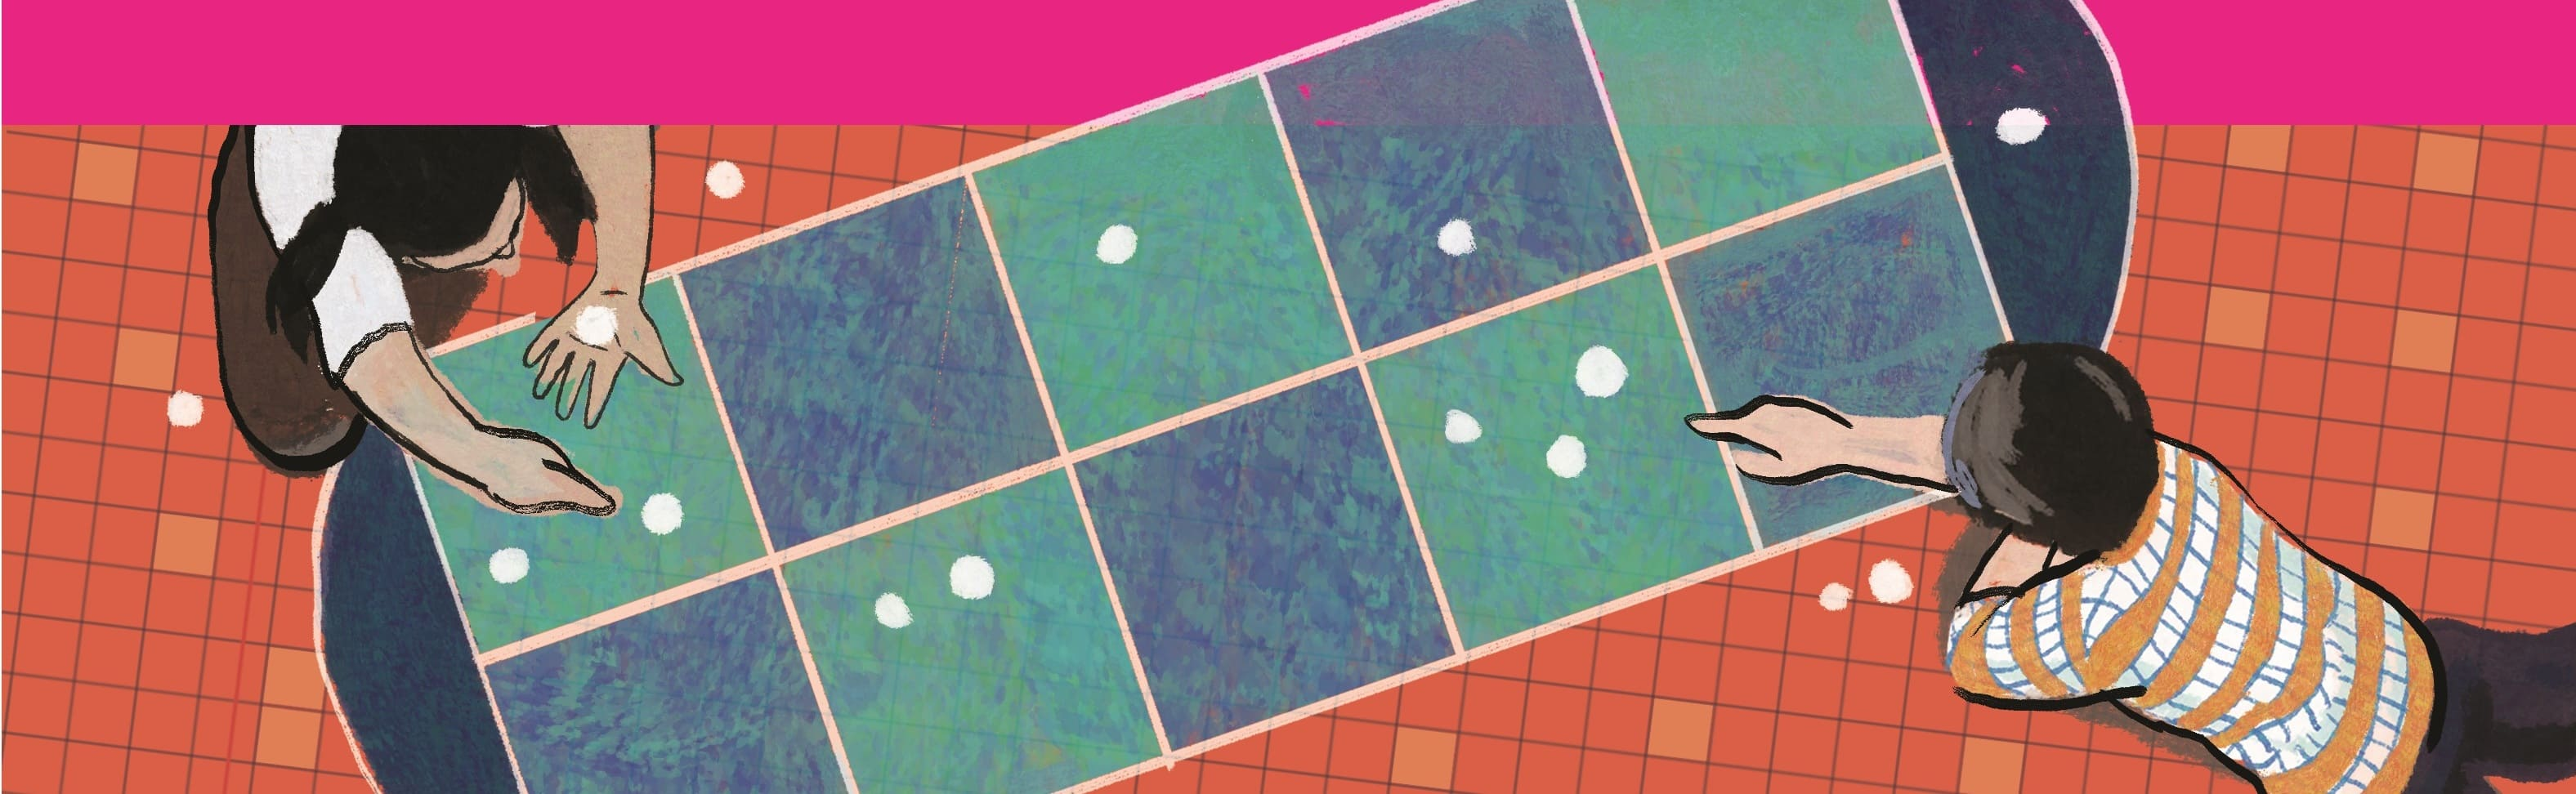
\includegraphics[width=19.3cm]{../bannertoancuabi}}}  
%\AddToShipoutPicture*{\put(80,495){\includegraphics[scale=1]{../tieudea.pdf}}}  
\centering
\endgroup
\vspace*{215pt} 

\definecolor{bulgarianrose}{rgb}{0.28, 0.02, 0.03}
%\begin{multicols}{2}
%	Các bạn nhỏ thân mến, tiếp tục với những bài giảng được dạy trong Câu lạc bộ Unicorn Math Circle (UMC), bài viết lần này giới thiệu về chủ đề Phép dời hình và ứng dụng trong việc xây dựng công thức tính diện tích của những hình thường gặp. Những phép dời hình cơ bản được giới thiệu trong chuỗi những bài viết là: Phép đối xứng trục hay phép phản xạ (reflection), phép đối xứng tâm (point reflection), phép quay (rotation) và phép tịnh tiến (translation).
%	\begin{figure}[H]
%		\vspace*{-5pt}
%		\centering
%		\captionsetup{labelformat= empty, justification=centering}
%		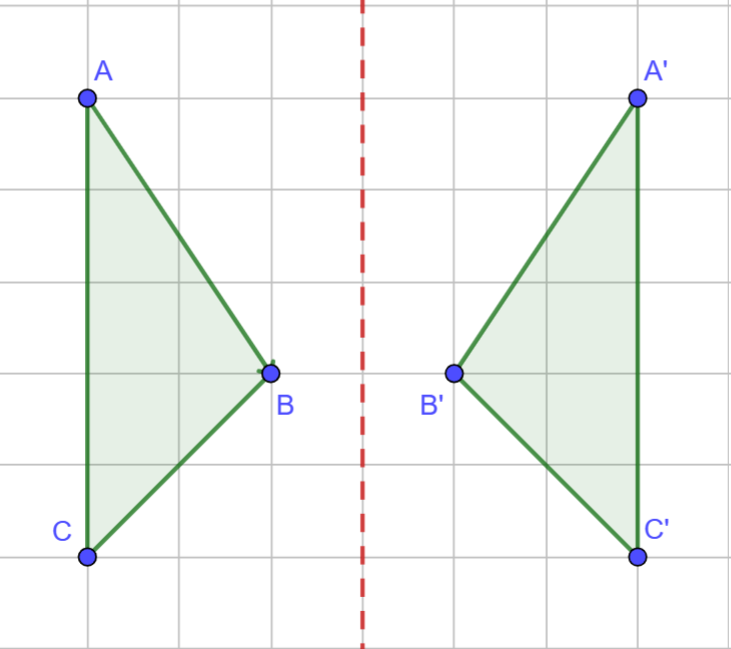
\includegraphics[width= 0.75\linewidth]{Hinh1}
%		\caption{\small\textit{\color{toancuabi}Hình $1$.}}
%		\vspace*{-10pt}
%	\end{figure}
%	Những phép dời hình được đề cập ở đây chỉ di chuyển hình mà không làm thay đổi hình dạng và kích thước của những hình đã cho và do đó những hình mới có diện tích không đổi so với hình cũ. Phép dời hình đầu tiên được giới thiệu trong bài viết này là phép phản xạ. Các phép dời hình còn lại được giới thiệu lần lượt trong các bài viết tiếp theo.
%	\vskip 0.1cm
%	Phép phản xạ tạo ra một hình mới bằng cách lật hình đã cho thành hình ảnh phản chiếu (mirror image) của nó.
%	\begin{figure}[H]
%		\vspace*{-5pt}
%		\centering
%		\captionsetup{labelformat= empty, justification=centering}
%		
\includegraphics[width= 1\linewidth]{Hinh2}
%		\caption{\small\textit{\color{toancuabi}Hình $2$.}}
%		\vspace*{-10pt}
%	\end{figure}
%	Trong Hình $1$ ở đây, tam giác $ABC$ bên trái bị phản xạ (hay lật) qua đường kẻ màu đỏ để tạo thành tam giác $A'B'C'$ bên phải. Hoặc có thể nói là các đỉnh $A,B,$ và $C$ của tam giác được phản xạ lên đường kẻ màu đỏ để tạo ra ảnh gương là một tam giác có đỉnh $A'$, $B'$, và $C'$ khác. Người ta gọi đường kẻ màu đỏ đó là trục phản xạ, trục đối xứng hay trục gương. Lưu ý rằng hình thứ $2$, gọi là ảnh, nằm ngược lại hoàn toàn với hình ban đầu. Các bạn nhỏ có thể dễ dàng nhớ điều này khi liên hệ tới chiếc gương: Hình ảnh trong gương phản chiếu mọi thứ, nhưng tất cả trong ảnh bị ngược lại so với thực tế.
%	\vskip 0.1cm
%	Phép phản xạ cũng được nhìn thấy ở nhiều hiện tượng trong thực tế. Cảnh mặt trời lặn xuống núi được phản xạ (soi bóng) xuống mặt sông là một trong những hình ảnh phản xạ rất đẹp trong cuộc sống.
%	\begin{figure}[H]
%		\vspace*{-5pt}
%		\centering
%		\captionsetup{labelformat= empty, justification=centering}
%		
\includegraphics[width= 1\linewidth]{Hinh3}
%		\caption{\small\textit{\color{toancuabi}Hình $3$.}}
%		\vspace*{-10pt}
%	\end{figure}
%	Do phép phản xạ chỉ lật hình qua một trục nên \textbf{\color{toancuabi}\color{toancuabi}hình ảnh phản xạ được giữ nguyên hình dáng và kích thước}. Điều này cho ta một kết luận quan trọng đó là: \textbf{\color{toancuabi}\color{toancuabi}Diện tích của hình phản xạ và hình đã cho là như nhau}. Chẳng hạn trong ví dụ trên tam giác ABC và tam giác phản xạ của nó là $A'B'C'$ có diện tích bằng nhau. Hơn nữa, quan sát hình đầu tiên, ta thấy rằng hai điểm $A$ và $A'$ có cùng khoảng cách tới trục phản xạ là $3$ đơn vị. Điều tương tự cũng đúng với điểm $B'$ cách $1$ đơn vị và điểm $C'$ cách $3$ đơn vị. Hơn nữa, ta cũng thấy đoạn thẳng nối $AA'$, $BB'$ hay $CC'$ đều vuông góc với trục phản xạ. Bất cứ khi nào một hình được phản xạ, thì mỗi cặp điểm tương ứng phải cách trục phản xạ một khoảng bằng nhau và đoạn thẳng nối cặp điểm này phải vuông góc với trục phản xạ.
%	\begin{figure}[H]
%		\vspace*{5pt}
%		\centering
%		\captionsetup{labelformat= empty, justification=centering}
%		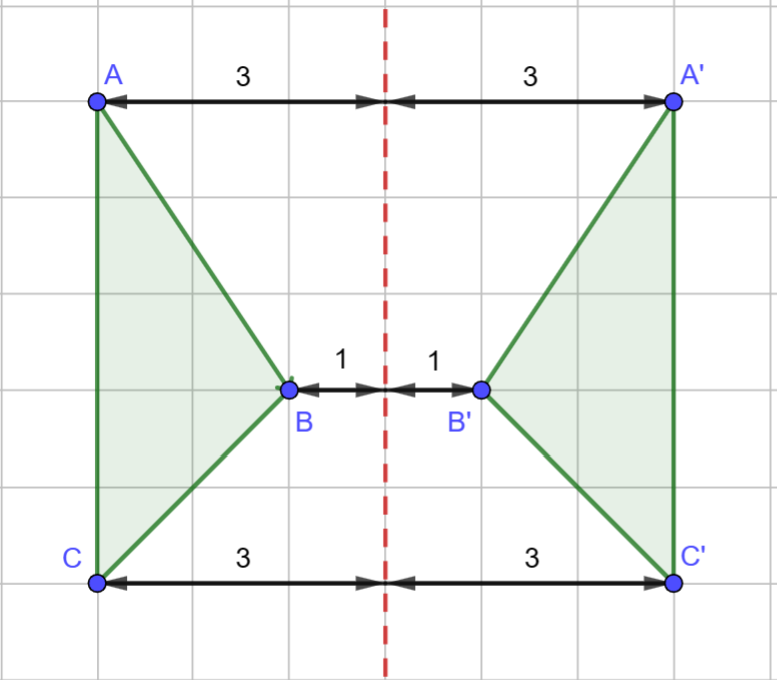
\includegraphics[width= 0.75\linewidth]{Hinh4}
%		\caption{\small\textit{\color{toancuabi}Hình $4$.}}
%		\vspace*{-10pt}
%	\end{figure}
%	Chúng ta cùng xem các ví dụ dưới đây để ôn lại những tính chất của phép phản xạ nhé.
%	\vskip 0.1cm 
%	\textbf{\color{toancuabi}\color{toancuabi}Ví dụ $\pmb{1}$.} Trong các hình cho dưới đây, cặp hình nào là phản xạ của nhau qua trục cho tương ứng?
%	\begin{figure}[H]
%		\vspace*{-5pt}
%		\centering
%		\captionsetup{labelformat= empty, justification=centering}
%		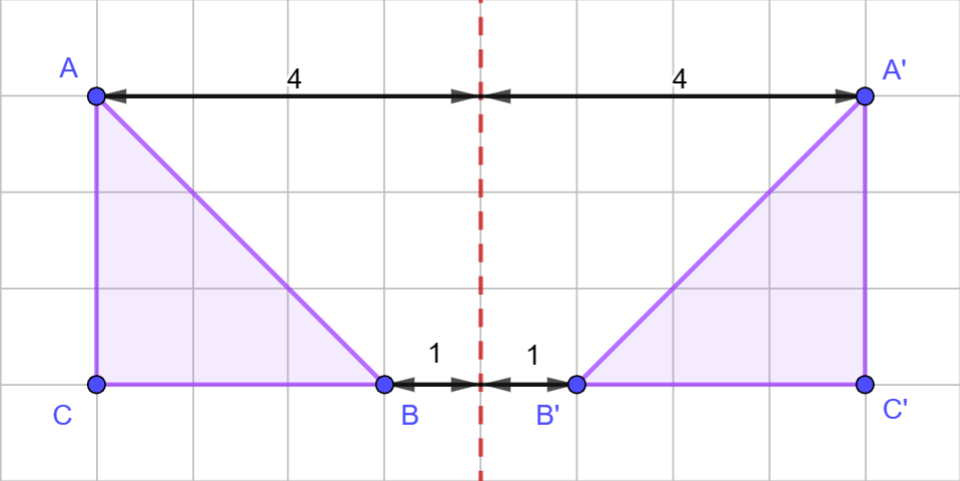
\includegraphics[width= 1\linewidth]{Hinh5}
%		\caption{\small\textit{\color{toancuabi}Hình $5$.}}
%		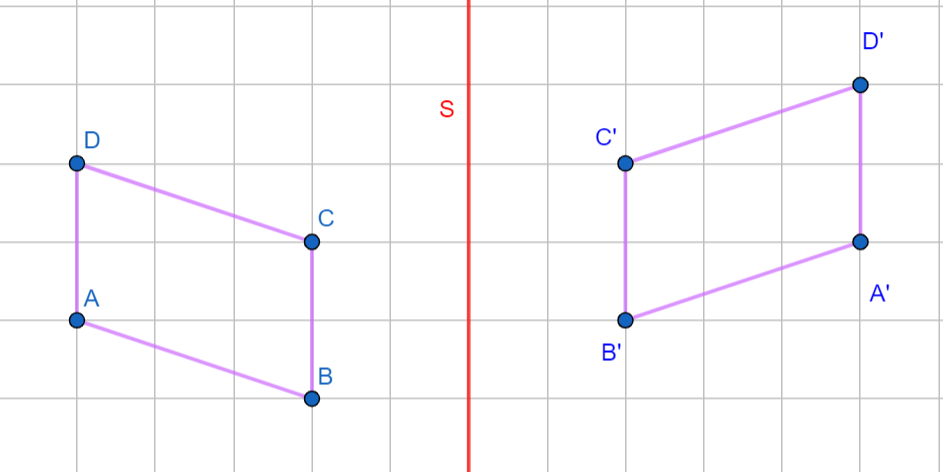
\includegraphics[width= 1\linewidth]{Hinh6}
%		\caption{\small\textit{\color{toancuabi}Hình $6$.}}
%		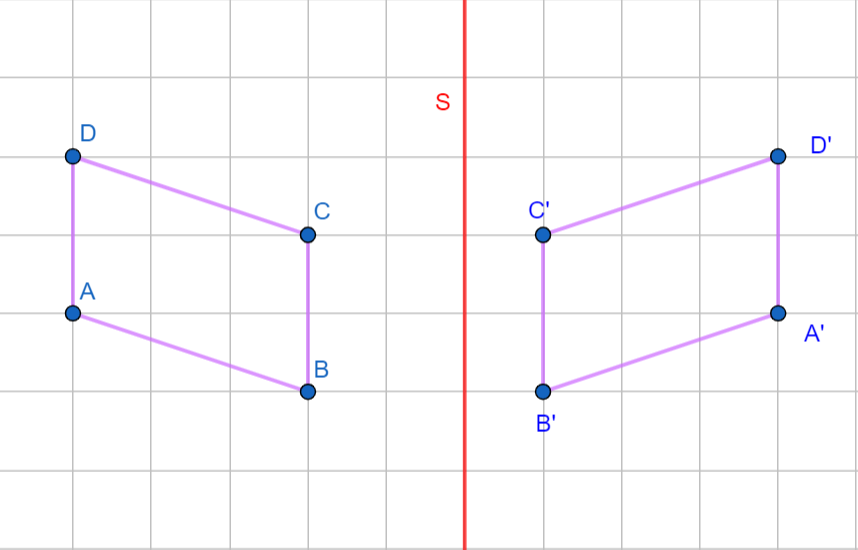
\includegraphics[width= 1\linewidth]{Hinh7}
%		\caption{\small\textit{\color{toancuabi}Hình $7$.}}
%		\vspace*{-5pt}
%	\end{figure}
%	\textit{Lời giải.}
%	Hình $5$ tam giác $A'B'C'$ là hình ảnh phản xạ của tam giác $ABC$ qua trục phản xạ $d$ vì các cặp điểm tương ứng $A$ và $A'$, $B$ và $B'$,  $C$ và $C'$ cùng cách đều trục $d$ và đoạn thẳng thẳng $AA'$, $BB'$,  $CC'$ vuông góc với trục $d$.
%	\vskip 0.1cm
%	Tuy nhiên, trong hai hình sau hình bình hành $A'B'C'D'$ không là hình phản xạ của hình bình hành $ABCD$ qua trục phản xạ $s$ bởi vì $AA'$ trong Hình $6$ không vuông góc với trục phản xạ và cặp điểm $A$, $A'$ không cách đều trục phản xạ trong Hình $7$.
%	\vskip 0.1cm
%	\textbf{\color{toancuabi}\color{toancuabi}Ví dụ} $\pmb{2}$. Hình chữ nhật A$'B'C'D'$ phải nằm ở vị trí nào để khi dùng phép phản xạ ta thu được hình chữ nhật $ABCD$?
%	\begin{figure}[H]
%		\vspace*{-5pt}
%		\centering
%		\captionsetup{labelformat= empty, justification=centering}
%		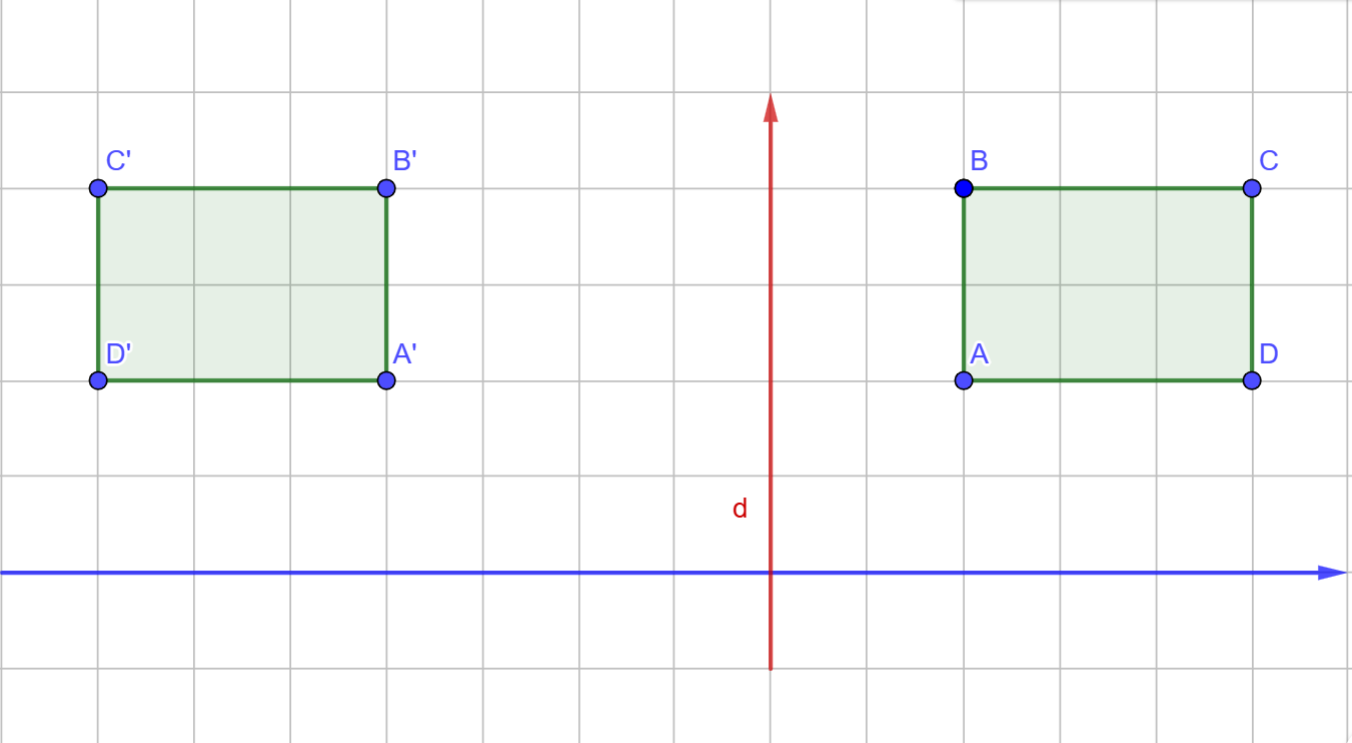
\includegraphics[width= 1\linewidth]{Hinh8}
%		\caption{\small\textit{\color{toancuabi}Hình $8$.}}
%		\vspace*{-10pt}
%	\end{figure}
%	\textit{Lời giải.}
%	Để $ABCD$ và $A'B'C'D'$ là  hình phản xạ của nhau thì trục phản xạ $d$ phải ở vị trí như trong Hình $9$ sau. Khi đó $AA'$ vuông góc $d$ và $A$,  $A'$ cùng cách $d$ một khoảng cách là $3$ đơn vị.
%	\begin{figure}[H]
%		\vspace*{-5pt}
%		\centering
%		\captionsetup{labelformat= empty, justification=centering}
%		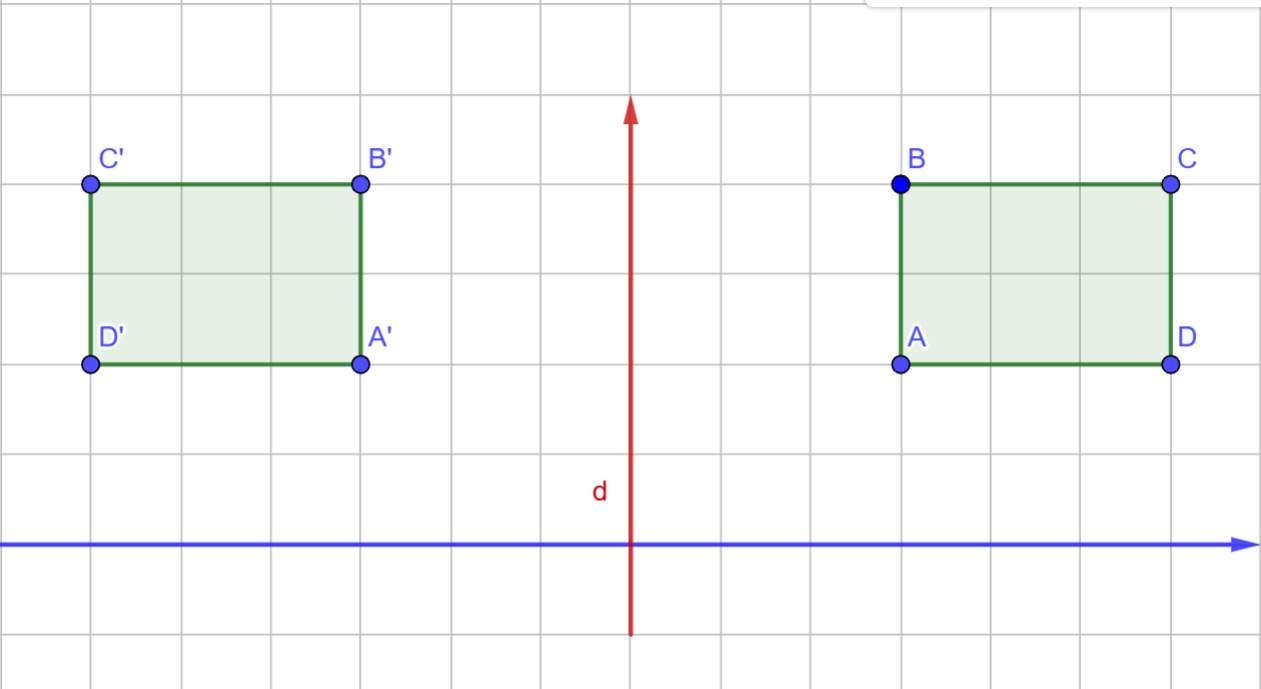
\includegraphics[width= 1\linewidth]{Hinh9}
%		\caption{\small\textit{\color{toancuabi}Hình $9$.}}
%		\vspace*{-10pt}
%	\end{figure}
%	\textbf{\color{toancuabi}\color{toancuabi}Ví dụ} $\pmb{3}.$ Vẽ một hình chữ nhật $ABCD$ có $AB=4\,cm$ và $AD=3\,cm$. Xác định ảnh phản xạ qua các trục đối xứng sau:
%	\vskip 0.1cm
%	$(a)$ Đoạn thẳng $AB$
%	\vskip 0.1cm
%	$(b)$ Đoạn thẳng $BC$
%	\vskip 0.1cm		
%	$(c)$ Đoạn thẳng $AC$
%	\vskip 0.1cm
%	\textit{Lời giải.}  
%	$(a)$ Ta xác định điểm $D'$ sao cho $A$ là trung điểm của đoạn $DD'$ và điểm $C'$ sao cho $B$ là trung điểm của đoạn $CC'$. Khi đó ảnh phản xạ của $ABCD$ qua đoạn AB là hình chữ nhật $ABC'D'$ được minh họa trong Hình $10$. 
%	\begin{figure}[H]
%		\vspace*{-5pt}
%		\centering
%		\captionsetup{labelformat= empty, justification=centering}
%		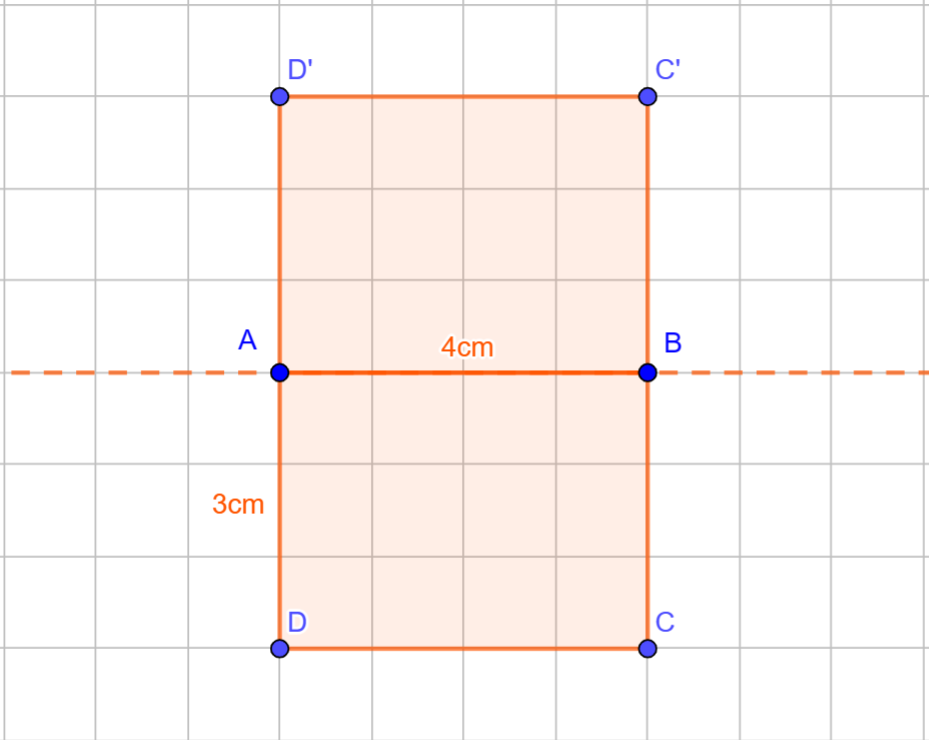
\includegraphics[width= 1\linewidth]{Hinh10}
%		\caption{\small\textit{\color{toancuabi}Hình $10$.}}
%		\vspace*{-10pt}
%	\end{figure}
%	$(b)$ Tương tự như câu $(a)$, ta xác định hai điểm $A'$ và $D'$ như Hình $11$. Vậy $A'BCD'$ là ảnh phản xạ của hình chữ nhật $ABCD$ qua $BC$. 
%	\begin{figure}[H]
%		\vspace*{-5pt}
%		\centering
%		\captionsetup{labelformat= empty, justification=centering}
%		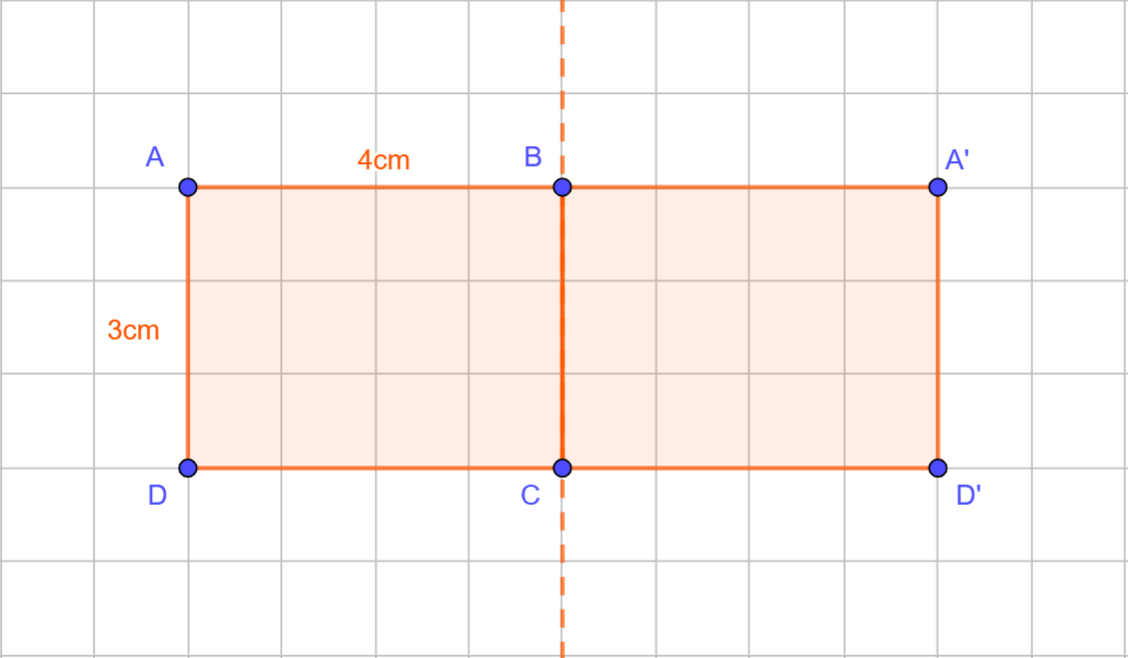
\includegraphics[width= 1\linewidth]{Hinh11}
%		\caption{\small\textit{\color{toancuabi}Hình $11$.}}
%		\vspace*{-10pt}
%	\end{figure}
%	$(c)$ Do $A$ và $C$ nằm trên trục phản xạ nên ta chỉ cần xác định ảnh phản xạ của hai điểm $B$ và $D$. Đầu tiên kẻ đường thẳng đi qua $D$ và vuông góc với trục $AC$ tại $E$. Sau đó xác định điểm $D'$ nằm trên đường thẳng đó sao cho độ dài $AD'$ bằng $3\,cm$. Làm tương tự với điểm $B$ ta sẽ thu được ảnh phản xạ là hình chữ nhật $AB'CD'$ như Hình $12$.
%	\begin{figure}[H]
%		\vspace*{5pt}
%		\centering
%		\captionsetup{labelformat= empty, justification=centering}
%		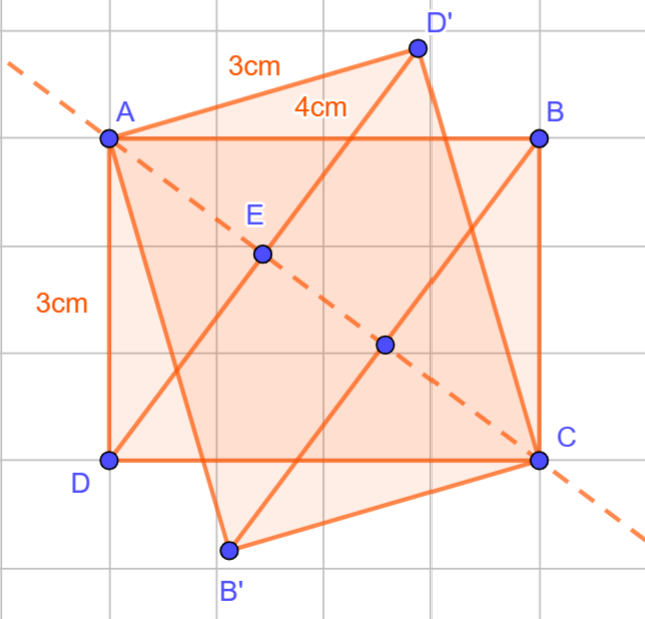
\includegraphics[width= 0.7\linewidth]{Hinh12}
%		\caption{\small\textit{\color{toancuabi}Hình $12$.}}
%		\vspace*{-10pt}
%	\end{figure}
%	\textbf{\color{toancuabi}\color{toancuabi}Ví dụ $\pmb4$.} Hình vuông trong Hình $13$ được tạo thành từ $25$ ô vuông, trong đó $6$ ô vuông trong hình đã được tô màu. Hãy tô thêm $3$ hình vuông nữa để hai nửa của hình vuông phản xạ với nhau qua trục đối xứng AB.
%	\begin{figure}[H]
%		\vspace*{-5pt}
%		\centering
%		\captionsetup{labelformat= empty, justification=centering}
%		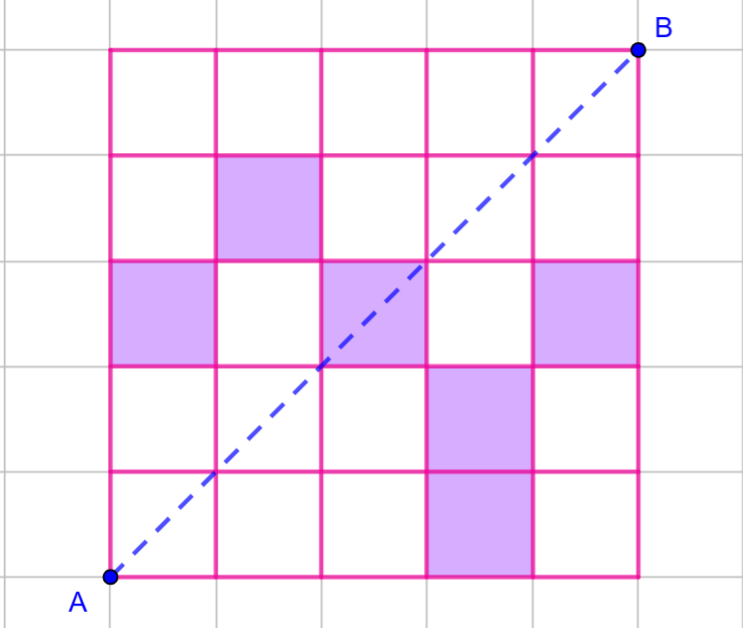
\includegraphics[width= 0.7\linewidth]{Hinh13}
%		\caption{\small\textit{\color{toancuabi}Hình $13$.}}
%		\vspace*{-10pt}
%	\end{figure}
%	\textit{Lời giải.} Ta cần chỉ ra ảnh phản xạ của từng ô vuông đơn vị qua trục $AB$ nằm ở vị trí nào trên hình. Rõ ràng ba ô vuông cần được tô màu nằm ở vị trí dòng $1$, cột $3$; dòng $5$, cột $3$ và dòng $2$ cột $1$ và Hình sau khi tô được vẽ  như trong Hình $14$.
%	\begin{figure}[H]
%		\vspace*{-5pt}
%		\centering
%		\captionsetup{labelformat= empty, justification=centering}
%		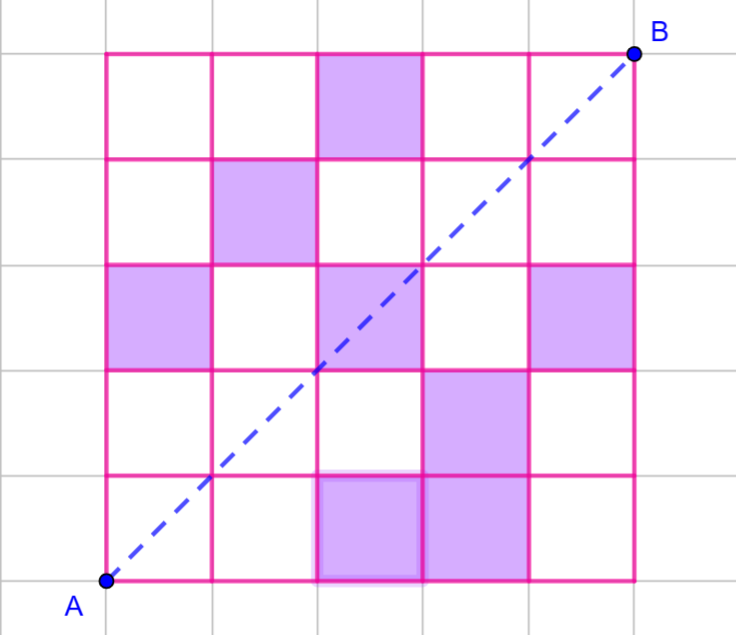
\includegraphics[width= 0.7\linewidth]{Hinh14}
%		\caption{\small\textit{\color{toancuabi}Hình $14$.}}
%		\vspace*{-5pt}
%	\end{figure}	
%	\textbf{\color{toancuabi}\color{toancuabi}Ví dụ $\pmb5$.} Vẽ một tam giác $ABC$ (Hình $F$) và đường thẳng $d$ trên một tờ giấy như trong Hình $15$. Gấp tờ giấy dọc theo đường thẳng $d$ và dùng một cây kim đâm xuyên qua ba đỉnh $A$, $B$ và $C$. Ký hiệu các điểm ở mặt giấy kia là $A',B',C'$ rồi nối chúng lại với nhau để tạo thành hình $F'$. Theo các bạn hình $F'$ có là ảnh phản xạ của $F$ qua đường thẳng $d$ hay không?
%	\begin{figure}[H]
%		\vspace*{-5pt}
%		\centering
%		\captionsetup{labelformat= empty, justification=centering}
%		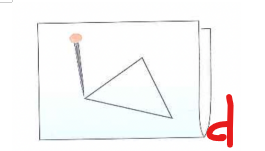
\includegraphics[width= 0.4\linewidth]{Hinh15.1}
%		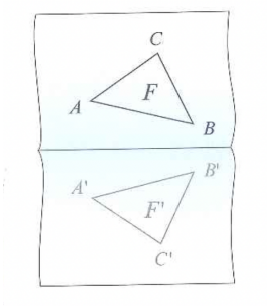
\includegraphics[width= 0.5\linewidth]{Hinh15.2}
%		\caption{\small\textit{\color{toancuabi}Hình $15$.}}
%		\vspace*{-10pt}
%	\end{figure}
%	\textit{Lời giải.} Hình $F'$ là ảnh phản xạ của $F$ qua trục phản xạ $d$ vì khi gấp tờ giấy theo đường thẳng $d$ thì $F'$ trùng khít với $F$,  hay $F$ được lật qua đường thẳng $d$ để thành hình $F'$.    
%	\vskip 0.1cm
%	Dưới đây là một số bài tập để các em luyện tập thêm về hình phản xạ và trục đối xứng trong phép phản xạ.
%	\vskip 0.1cm
%	\textbf{\color{toancuabi}\color{toancuabi}Bài tập $\pmb1$.} Hãy vẽ ảnh phản xạ của hình bình hành qua trục phản xạ trong Hình $16$.
%	\begin{figure}[H]
%		\vspace*{-5pt}
%		\centering
%		\captionsetup{labelformat= empty, justification=centering}
%		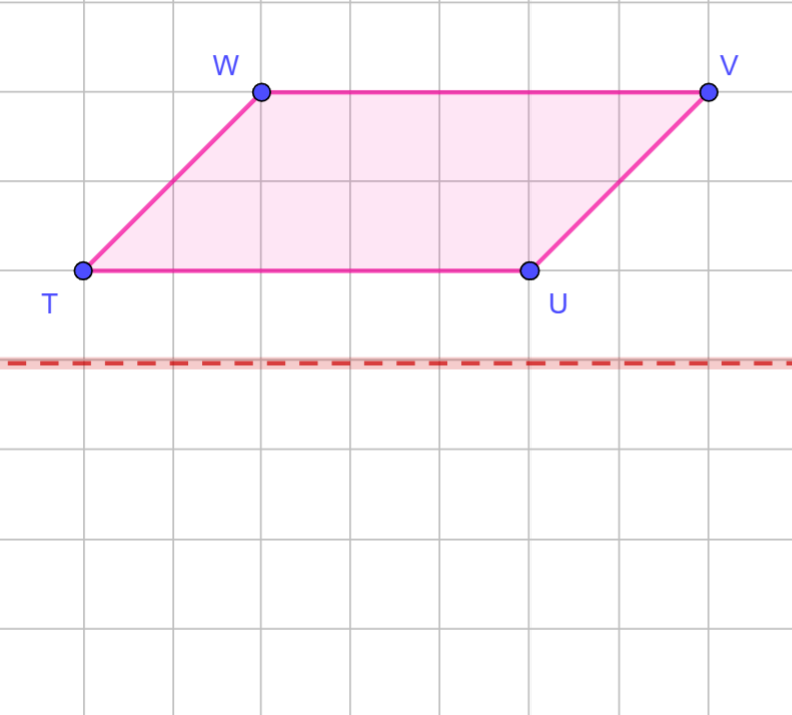
\includegraphics[width= 0.75\linewidth]{Hinh16}
%		\caption{\small\textit{\color{toancuabi}Hình $16$.}}
%		\vspace*{-10pt}
%	\end{figure}
%	\textbf{\color{toancuabi}\color{toancuabi}Bài tập $\pmb2$.} Một hình chữ nhật $A$ được phản xạ để tạo ra hình chữ nhật B như trong Hình $17$. Hãy xác định trục đối xứng.
%	\begin{figure}[H]
%		\vspace*{5pt}
%		\centering
%		\captionsetup{labelformat= empty, justification=centering}
%		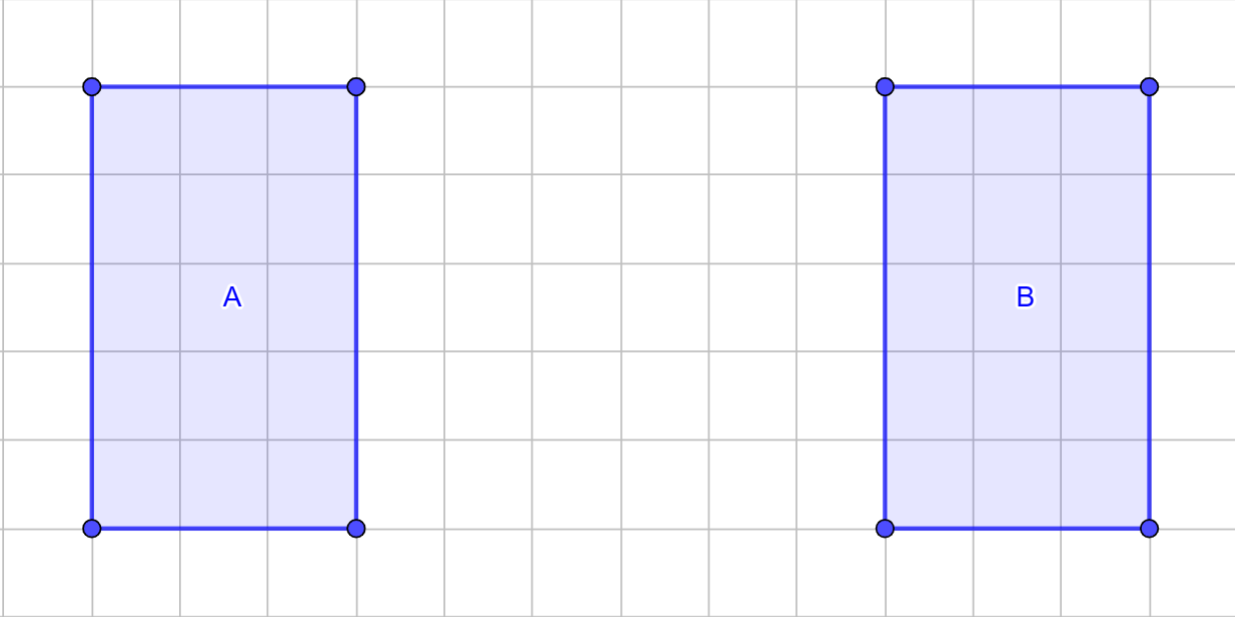
\includegraphics[width= 1\linewidth]{Hinh17}
%		\caption{\small\textit{\color{toancuabi}Hình $17$.}}
%		\vspace*{-10pt}
%	\end{figure}
%	\textbf{\color{toancuabi}\color{toancuabi}Bài tập $\pmb3$}: Hình $F'$ có là ảnh phản xạ của $F$ qua đường thẳng $s$ trong các trường hợp trong Hình $18$ dưới đây hay không?
%	\begin{figure}[H]
%		\vspace*{-5pt}
%		\centering
%		\captionsetup{labelformat= empty, justification=centering}
%		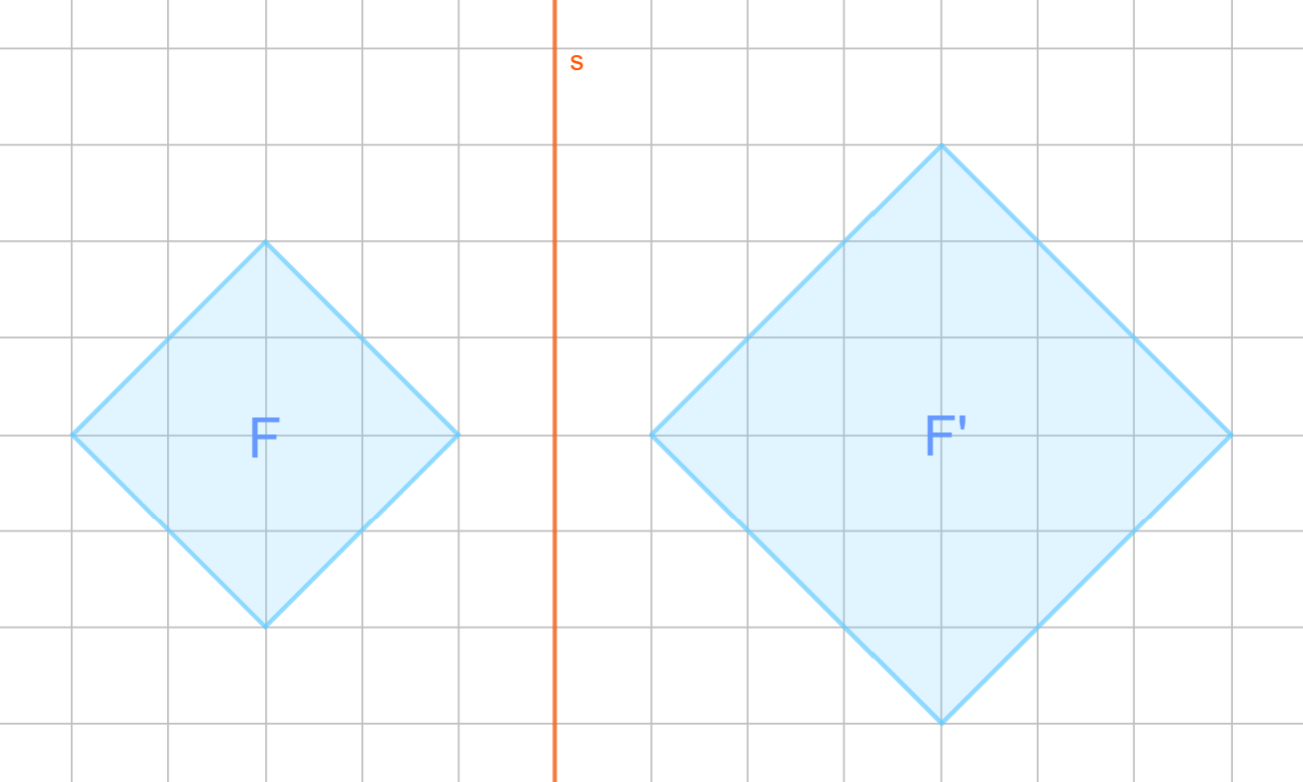
\includegraphics[width= 0.8\linewidth]{Hinh18.1}
%		
%		\vspace*{5pt}
%		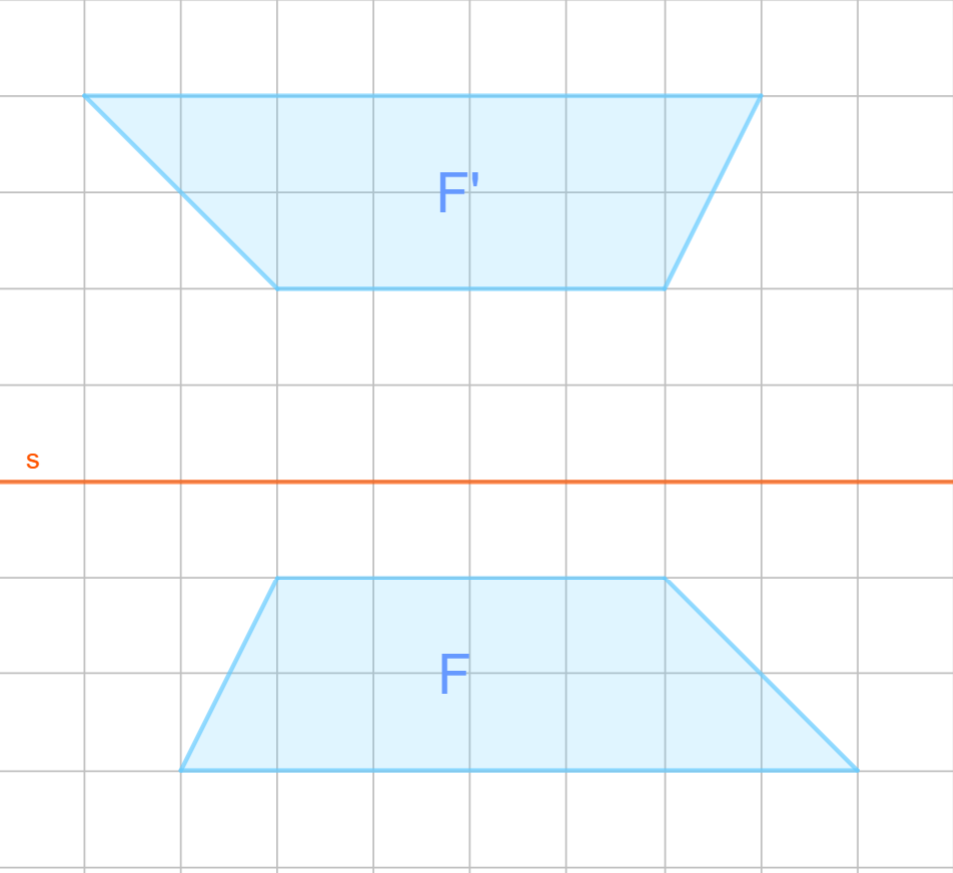
\includegraphics[width= 0.76\linewidth]{Hinh18.2}
%		
%		\vspace*{5pt}
%		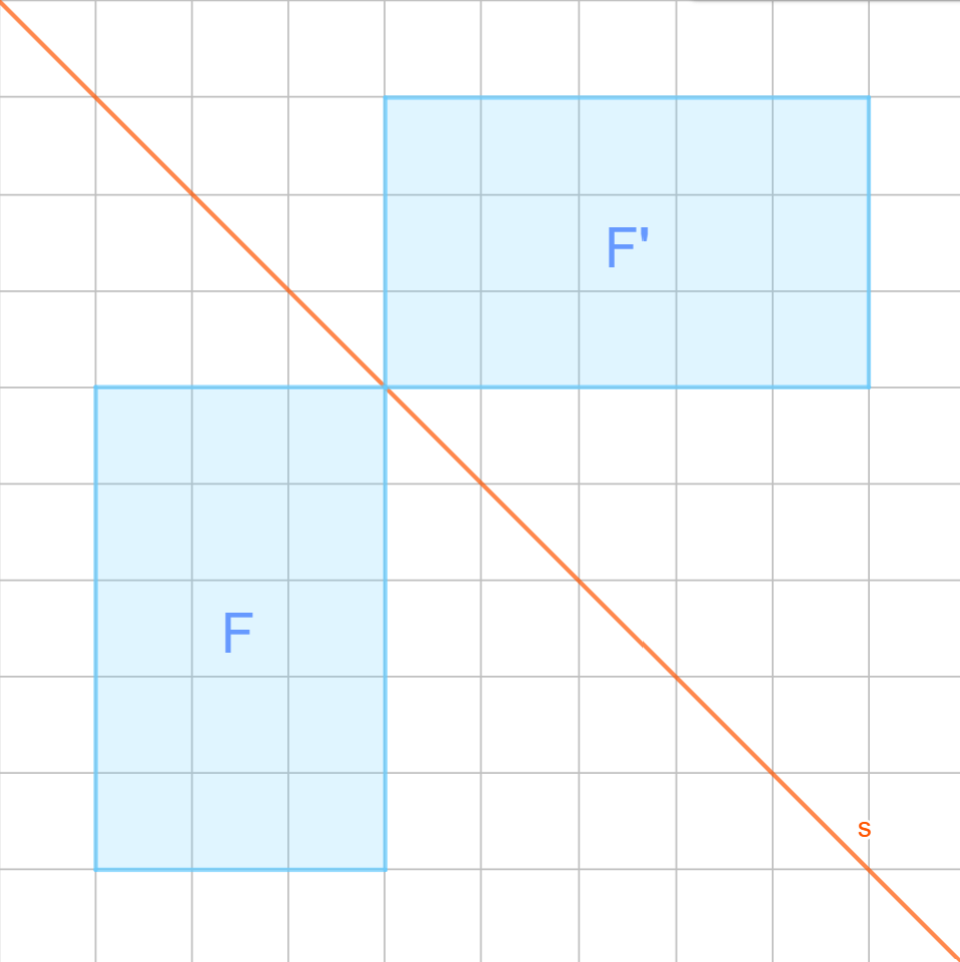
\includegraphics[width= 0.75\linewidth]{Hinh18.3}
%		\caption{\small\textit{\color{toancuabi}Hình $18$.}}
%		\vspace*{-10pt}
%	\end{figure}
%	\textbf{\color{toancuabi}\color{toancuabi}Bài tập $\pmb4$.} Vẽ trục đối xứng $d$ của hai điểm $A$ và $A'$. Sau đó vẽ ảnh phản xạ của các hình trong Hình $19$ qua $d$.
%	\begin{figure}[H]
%		\vspace*{-5pt}
%		\centering
%		\captionsetup{labelformat= empty, justification=centering}
%		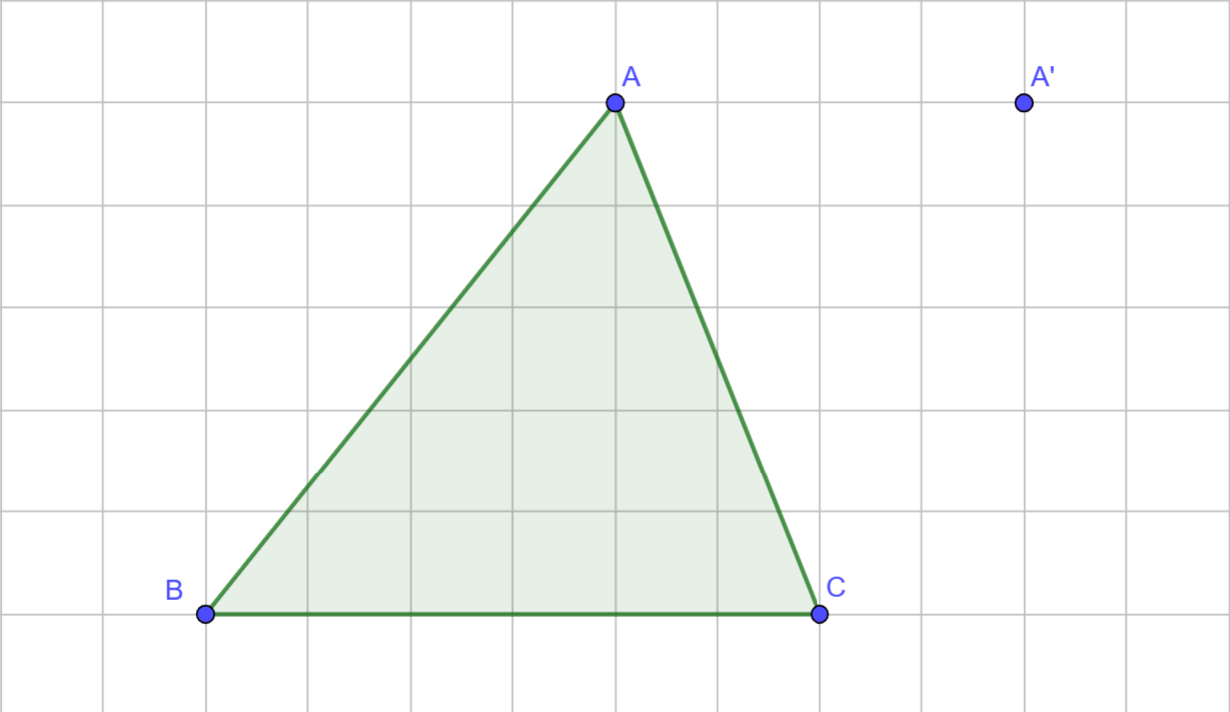
\includegraphics[width= 1\linewidth]{Hinh19.1}
%		
%		\vspace*{5pt}
%		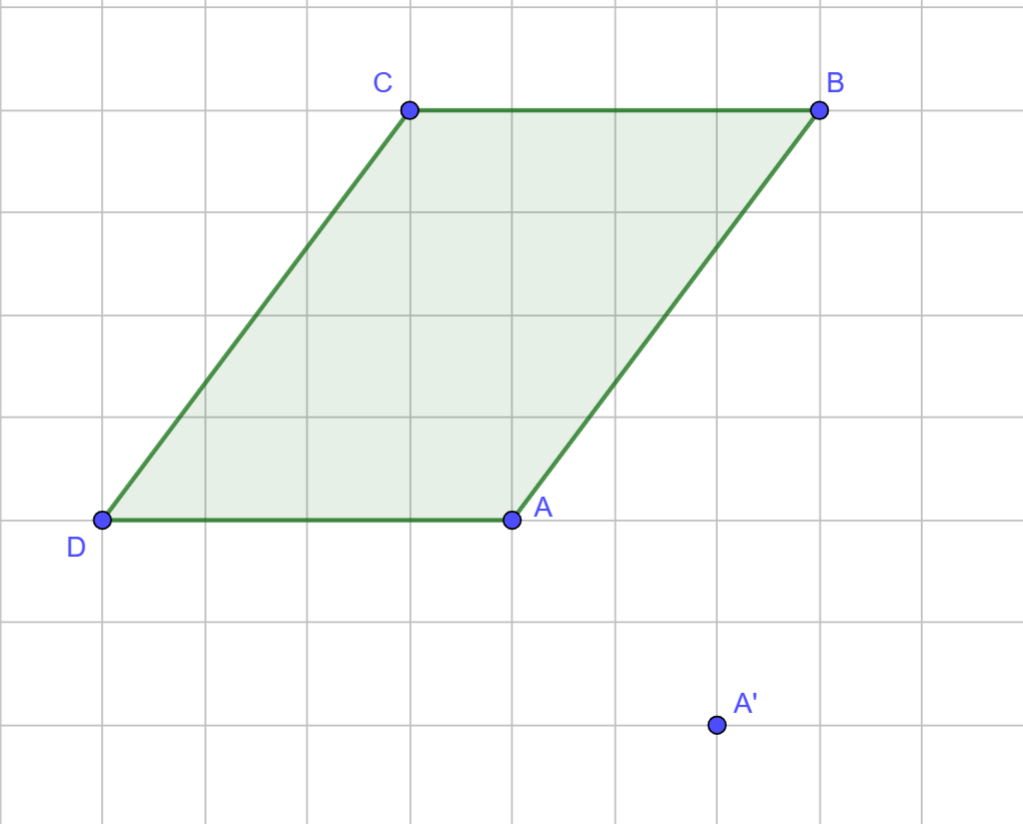
\includegraphics[width= 1\linewidth]{Hinh19.2}
%		\caption{\small\textit{\color{toancuabi}Hình $19$.}}
%		\vspace*{-10pt}
%	\end{figure}
%	\textbf{\color{toancuabi}\color{toancuabi}Bài tập $\pmb5$.} Hãy tô thêm đúng hai ô vuông nữa để hình vuông trong Hình $20$ có đúng hai trục đối xứng.
%	\begin{figure}[H]
%		\vspace*{-5pt}
%		\centering
%		\captionsetup{labelformat= empty, justification=centering}
%		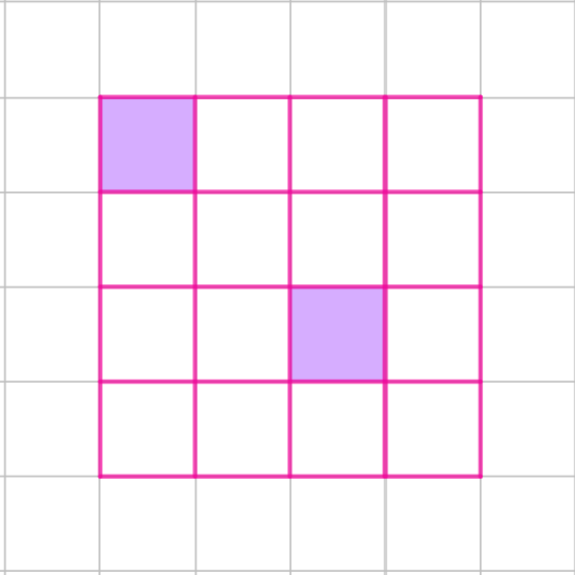
\includegraphics[width= 0.75\linewidth]{Hinh20}
%		\caption{\small\textit{\color{toancuabi}Hình $20$.}}
%		\vspace*{-10pt}
%	\end{figure}
%\end{multicols}
%\newpage
%\begingroup
%\AddToShipoutPicture*{\put(66,635){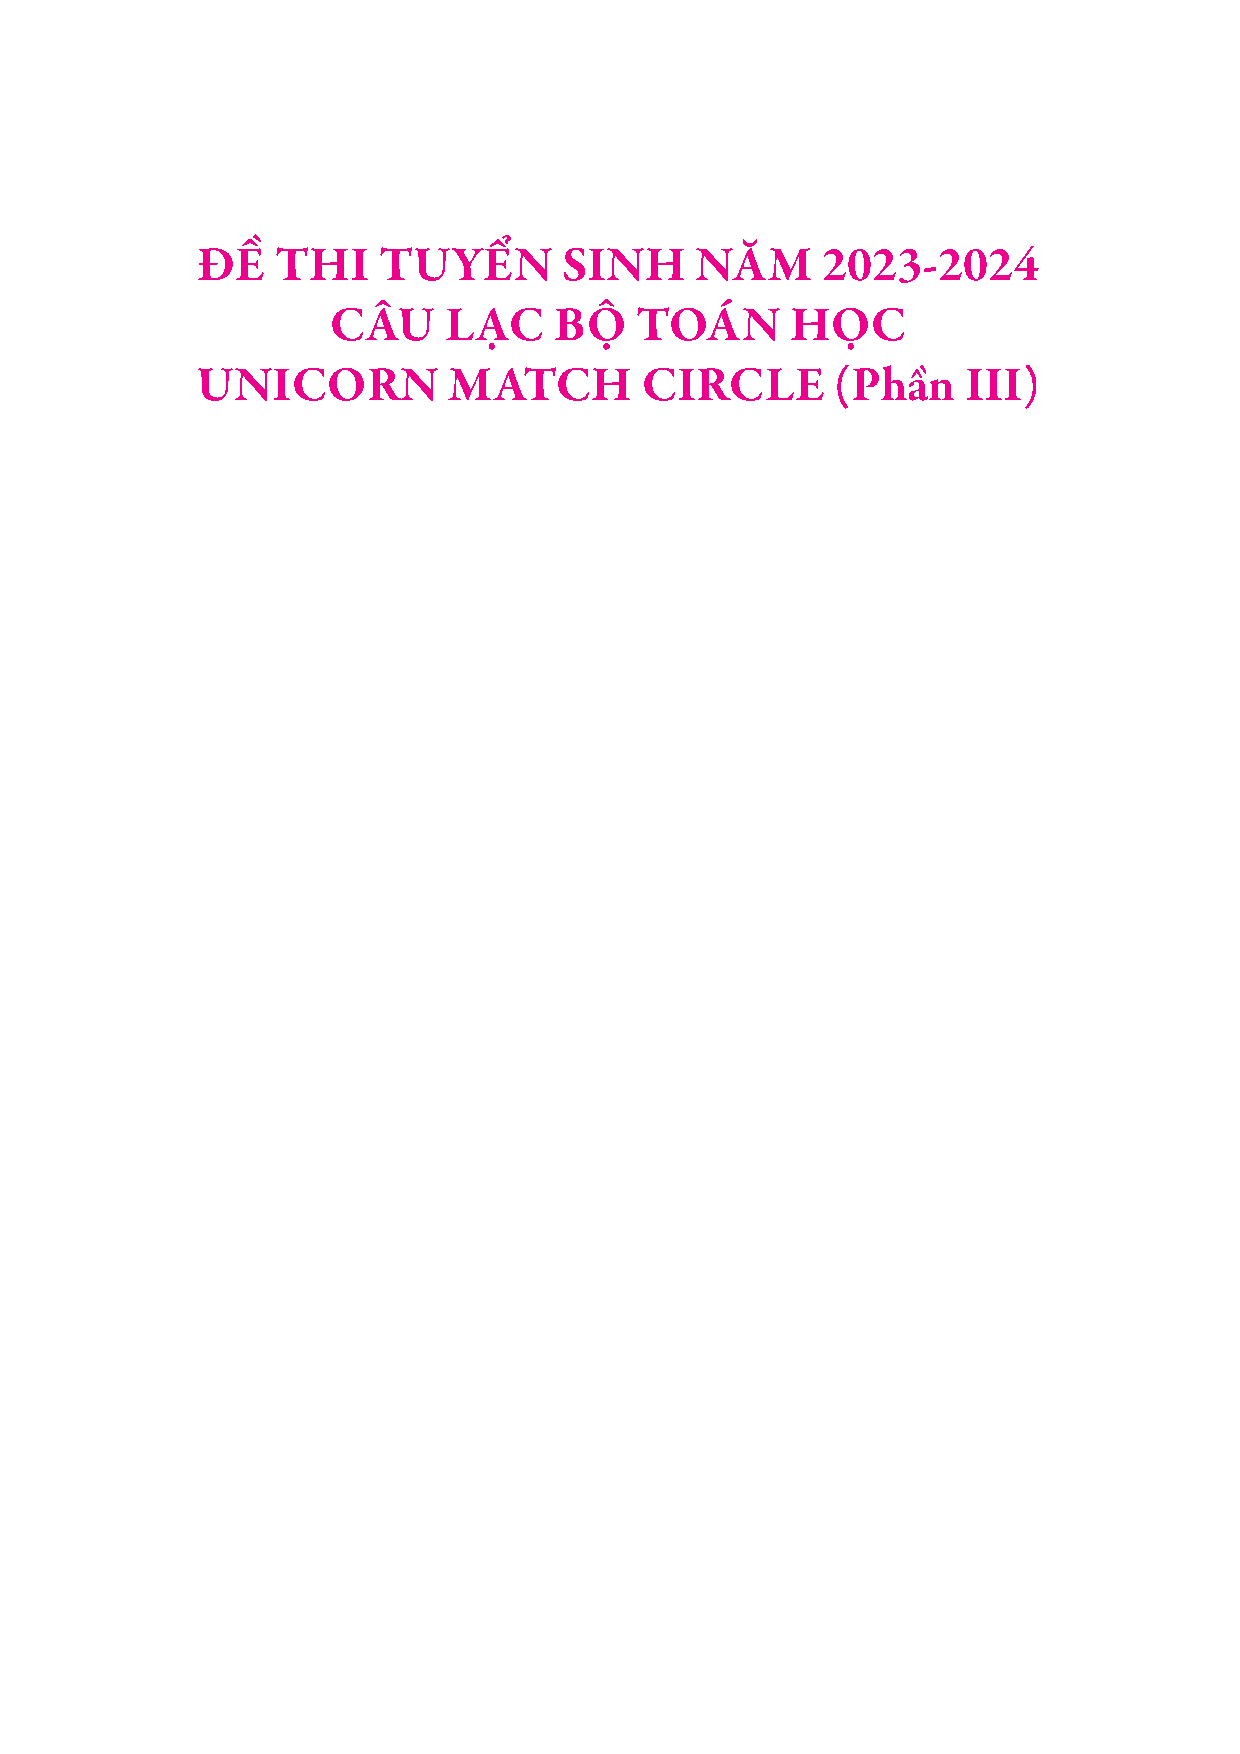
\includegraphics[scale=1]{../tieude1.pdf}}} 
%\centering
%\endgroup
%\vspace*{70pt}
%
%\begin{multicols}{2}
%	Tiếp tục với nội dung về đề thi tuyển sinh vào Câu lạc bộ Unicorn Math Circle, trong số này, tạp chí Pi giới thiệu đến bạn đọc bài thi dành cho các bạn học sinh lớp $6$. Thời gian đề xuất làm bài là $90$ phút. 
%	\vskip 0.1cm
%	\textbf{\color{toancuabi}\color{toancuabi}Bài $\pmb1$.} Trong một chiếc hộp kín có $7$ quả bóng xanh, $8$ quả bóng đỏ và $9$ quả bóng vàng. Hỏi cần lấy ra ngẫu nhiên ít nhất bao nhiêu quả bóng để chắc chắn có $2$ quả bóng mỗi màu?
%	\vskip 0.1cm
%	\textbf{\color{toancuabi}\color{toancuabi}Bài $\pmb2$.} Xét dãy hình dưới đây. Dựa vào quy luật, hãy cho biết có bao nhiêu hình tam giác trong $2023$ hình đầu tiên tính từ trái sang?
%	\begin{figure}[H]
%		\vspace*{-5pt}
%		\centering
%		\captionsetup{labelformat= empty, justification=centering}
%		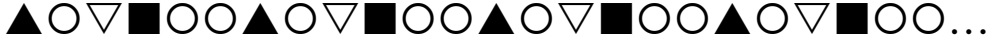
\includegraphics[width= 1\linewidth]{1}
%%		\caption{\small\textit{\color{}}}
%		\vspace*{-10pt}
%	\end{figure}
%	\textbf{\color{toancuabi}\color{toancuabi}Bài $\pmb3$.} Trên bảng ta viết liên tiếp các số tự nhiên từ $1$ tới $500$. Tiếp theo, ta gạch đi tất cả các số là bình phương hoặc là lập phương của một số nguyên. Hỏi trong các số còn lại trên bảng không được xoá, số đứng ở vị trí thứ $105$ là số nào?
%	\vskip 0.1cm
%	\textbf{\color{toancuabi}\color{toancuabi}Bài $\pmb4$.} Trong một câu lạc bộ văn nghệ chỉ có $1/7$ thành viên là các bạn nam. Sau khi có thêm $13$ bạn đăng ký thì số bạn nam trong nhóm tăng lên, tuy nhiên tỷ lệ các thành viên nam so với thành viên nữ trong nhóm lại giảm đi. Hỏi số lượng các bạn nữ được bổ sung mới vào câu lạc bộ là bao nhiêu?
%	\vskip 0.1cm
%	\textbf{\color{toancuabi}\color{toancuabi}Bài $\pmb5$.} Có bao nhiêu số có $3$ chữ số khác nhau, chia hết cho $11$, được tạo thành từ các chữ số $1, 3, 5, 7, 9$?
%	\vskip 0.1cm
%	\textbf{\color{toancuabi}\color{toancuabi}Bài $\pmb6$.} Biết rằng mỗi ô vuông trên lưới có cạnh là $1$ đơn vị. Hỏi hình được tô đậm dưới đây có diện tích là bao nhiêu?
%	\begin{figure}[H]
%		\vspace*{5pt}
%		\centering
%		\captionsetup{labelformat= empty, justification=centering}
%		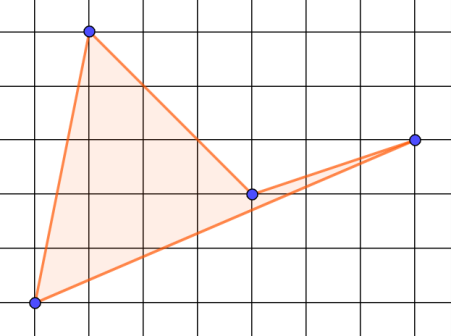
\includegraphics[width= 1\linewidth]{2}
%		%		\caption{\small\textit{\color{}}}
%		\vspace*{-15pt}
%	\end{figure}
%%	\begin{figure}[H]
%%		\vspace*{-5pt}
%%		\centering
%%		\captionsetup{labelformat= empty, justification=centering}
%%		\begin{tikzpicture}
%%			\draw (0,0) grid (9,8);
%%			\draw (1,1) node[fill = gocco] circle (2pt);
%%			\draw (2,6) node[fill = gocco] circle (2pt);
%%			\draw (5,3) node[fill = gocco] circle (2pt);
%%			\draw (8,4) node[fill = gocco] circle (2pt);
%%		\end{tikzpicture}
%%%		\caption{\small\textit{\color{}}}
%%		\vspace*{-10pt}
%%	\end{figure}
%	\textbf{\color{toancuabi}\color{toancuabi}Bài $\pmb7$.} Mỗi ngày bạn An có thể ăn $2$ hoặc $3$ viên kẹo. Hỏi có bao nhiêu cách khác nhau để bạn An ăn hết $13$ viên kẹo? Biết rằng các viên kẹo giống hệt nhau.
%	\vskip 0.1cm
%	\textbf{\color{toancuabi}\color{toancuabi}Bài $\pmb8$.} Một phần của một cuốn sách bị rơi ra, trong đó trang đầu tiên là $659$ và trang cuối cùng có số trang cũng gồm các chữ số $6,5,9$ nhưng được viết theo một thứ tự khác. Hỏi có bao nhiêu trang đã rơi ra?
%	\vskip 0.1cm
%	\textbf{\color{toancuabi}\color{toancuabi}Bài $\pmb9$.} Trong một cuộc thi toán, đề thi gồm có $20$ câu hỏi, nếu thí sinh trả lời đúng $1$ câu sẽ được cộng $5$ điểm, trả lời sai một câu sẽ bị trừ $2$ điểm và phải đưa ra câu trả lời cho tất cả các câu hỏi. Biết rằng bạn An được $79$ điểm. Hỏi bạn An đã trả lời đúng bao nhiêu câu hỏi?
%	\vskip 0.1cm
%	\textbf{\color{toancuabi}\color{toancuabi}Bài $\pmb{10}$.} Trong một văn phòng có $6$ nhân viên. Mỗi người trong số họ có thể là người Thật thà (người luôn nói sự thật) hoặc kẻ Dối trá (người luôn nói dối). Một hôm $6$ người ngồi họp xung quanh một chiếc bàn tròn và mỗi người đều nói: ``Trong số ba người gồm hai người ngồi cạnh tôi và người ngồi đối diện với tôi qua tâm bàn tròn, có đúng hai kẻ Dối trá". Hỏi trong văn phòng có bao nhiêu người Thật thà?
%	\begin{figure}[H]
%		\vspace*{-5pt}
%		\centering
%		\captionsetup{labelformat= empty, justification=centering}
%		
\includegraphics[width= 1\linewidth]{3}
%		\vspace*{-10pt}
%	\end{figure}
%	\textbf{\color{toancuabi}\color{toancuabi}Đáp án}
%	\vskip 0.1cm
%	\textbf{\color{toancuabi}\color{toancuabi}Bài $\pmb1$.} 
%	Ta thấy số bóng đỏ và bóng vàng là lớn nhất, nên ta cần lấy ra ngẫu nhiên ít nhất $8+9+2=19$ (quả bóng) để sau khi lấy tổng số bóng lấy ra trừ đi tổng số bóng đỏ và vàng tối đa có thể lấy được, còn lại $2$ quả bóng xanh. 
%	\vskip 0.1cm
%	\textbf{\color{toancuabi}\color{toancuabi}Bài $\pmb2$.} 
%	Ta thấy dãy hình gồm các nhóm gồm $6$ hình 
%	\begin{figure}[H]
%		\vspace*{-5pt}
%		\centering
%		\captionsetup{labelformat= empty, justification=centering}
%		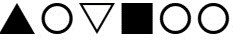
\includegraphics[width= 0.6\linewidth]{4}
%%		\caption{\small\textit{\color{}}}
%		\vspace*{-10pt}
%	\end{figure}
%	được sắp xếp liên tiếp nhau, trong mỗi nhóm hình có $2$ hình tam giác. Do $2023$ chia $6$ bằng $337$ dư $1$, nên trong $2023$ hình đầu tiên tính từ trái sang có số hình tam giác là: $337×2+1=675$.
%	\vskip 0.1cm
%	\textbf{\color{toancuabi}\color{toancuabi}Bài $\pmb3$.} 
%	Trong số $100$ số nguyên dương đầu tiên có $10$ số là bình phương của một số nguyên (từ $1^2=1$ tới $10^2=100$), và $4$ số là lập phương của một số nguyên (từ $1^3=1$ cho tới $4^3=64$).
%	\vskip 0.1cm
%	Các số $1$ và $64$ đồng thời vừa là số chính phương và là lập phương đúng của một số nguyên. Vì vậy, theo nguyên lý bao hàm -- loại trừ, trong $100$ số đầu tiên, ta đã gạch đi $10+4-2=12$ số.
%	\vskip 0.1cm
%	Trong $17$ số tiếp theo  từ $101$ tới $117$ không có số nào là bình phương hoặc lập phương của một số nguyên, do $11^2=121$ và $5^3=125$. Vì vậy trong các số còn lại trên bảng không được xoá, số đứng ở vị trí thứ $105$ là $105+12=117$.
%	\vskip 0.1cm
%	\textbf{\color{toancuabi}\color{toancuabi}Bài $\pmb4$.} Gọi số bạn nam là $x$. Vì số bạn nam chiếm $1/7$ tổng số thành viên, nên tổng số thành viên của câu lạc bộ sẽ là $7x$. Do đó số bạn nữ là 6x. Ta gọi số bạn nữ được bổ sung mới vào câu lạc bộ là a. Khi đó số bạn nam được bổ sung mới vào câu lạc bộ sẽ là $13-a$. Theo đề bài ta có: $13-a>0$, tức là $a<13$. Hơn nữa
%	\begin{align*}
%		\dfrac{x+ 13 - a}{6x + a} < \frac{1}{6} &\Rightarrow 6(x + 13 - a) < 6x + a\\
%		&\Rightarrow 7a > 78 \Rightarrow a > 11
%	\end{align*}
%	Từ đó $a=12$.
%	\vskip 0.1cm
%	Vậy có $12$ bạn nữ được bổ sung mới vào câu lạc bộ.
%	\vskip 0.1cm
%	\textbf{\color{toancuabi}\color{toancuabi}Bài $\pmb5$.} Giả sử $\overline{abc}$ là một số thỏa mãn điều kiện đề bài. Theo dấu hiệu chia hết cho $11$ ta có: $a+c-b$ chia hết cho $11$. Vì ta lấy $a,b,c$ là các chữ số khác nhau trong tập $\{1,3,5,7,9\}$, nên $a+c-b$ chỉ có thể bằng $11$.  Do đó $b=a+c-11$.
%	\vskip 0.1cm
%	Mà $a+c<9+9=18$, nên $b<18-11=7$. Do đó $b=1;3;5$.
%	\vskip 0.1cm
%	-- Khi $b=1 \Rightarrow a + c = 12 \Rightarrow a=5, c = 7$ hoặc $a= 7, c= 5$,  hoặc $a=3$, $c=9$ hoặc $a=9$, $c=3$. Ta được $4$ số.
%	\vskip 0.1cm
%	-- Khi $b=3\Rightarrow a + c = 14 \Rightarrow a =5, c = 9$ hoặc  $a = 9, c= 5$. Ta được $2$ số.
%	\vskip 0.1cm
%	-- Khi $b=5\Rightarrow a + c = 16 \Rightarrow a = 7, c= 9$ hoặc $a=9,c=7$. Ta được $2$ số.
%	\vskip 0.1cm
%	Vậy tổng cộng ta được $8$ số thỏa mãn yêu cầu đề bài. 
%	\vskip 0.1cm
%	\textbf{\color{toancuabi}\color{toancuabi}Bài $\pmb6$.} 
%	\begin{figure}[H]
%		\vspace*{5pt}
%		\centering
%		\captionsetup{labelformat= empty, justification=centering}
%		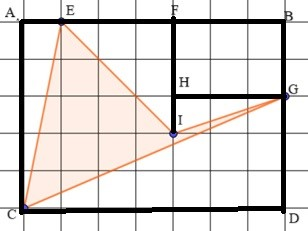
\includegraphics[width= 1\linewidth]{5}
%%		\caption{\small\textit{\color{}}}
%		\vspace*{-10pt}
%	\end{figure}
%	Ta thấy: Diện tích phần tô đậm bằng 
%	\begin{align*}
%		&S_{ABCD}-S_{EAC}-S_{GDC}-S_{GHI}\\
%		&-S_{BGHF}-S_{IFE}\\
%		=\,&5\times7-\frac{1\times5}{2}-\dfrac{3\times7}{2}-\frac{1\times3}{2}\\
%		&7-2\times3-\dfrac{3\times3}{2}\\
%		=&\,10.
%	\end{align*}
%	\textbf{\color{toancuabi}\color{toancuabi}Bài $\pmb7$.} Gọi $x$ là số ngày bạn An ăn $2$ viên kẹo và $y$ là số ngày bạn An ăn $3$ viên kẹo, với $x,y$ là các số nguyên dương. Khi đó ta có:
%	$2x+3y=13$. Từ đây ta suy ra y phải là số lẻ.
%	Mặt khác  . Do đó $y=1$ hoặc $y=3$.
%	\vskip 0.1cm
%	--Nếu $y=1$, thì  $x = \dfrac{13 - 3 \cdot1}{2} = 5$. Tức là có $5$ ngày bạn An ăn $2$ viên kẹo và $1$ ngày bạn An ăn $3$ viên kẹo. Số cách khác nhau để bạn An ăn các viên kẹo như vậy là $C_6^4$ (cách).
%	\vskip 0.1cm
%	-- Nếu $y=3$, thì  $x = \dfrac{13 - 3\cdot3}{2} = 2$. Tức là có $2$ ngày bạn An ăn $2$ viên kẹo và $3$ ngày bạn An ăn $3$ viên kẹo. Số cách khác nhau để bạn An ăn các viên kẹo như vậy là $C_5^2$ (cách).
%	\vskip 0.1cm
%	Vậy có tất cả $6+10=16$ cách khác nhau để bạn An ăn hết $13$ viên kẹo.
%	\vskip 0.1cm
%	\textbf{\color{toancuabi}\color{toancuabi}Bài $\pmb8$.} Vì trang cuối cùng cũng có số trang gồm các chữ số $6,5,9$ và phải là số chẵn nên trang cuối cùng sẽ có số trang là $956$. Như vậy số trang đã rơi ra là: $956-659+1=298$.
%	\vskip 0.1cm
%	\textbf{\color{toancuabi}\color{toancuabi}Bài $\pmb9$.} Gọi số câu bạn An trả lời đúng là $x$, khi đó số câu bạn An trả lời sai là $20-x$. Ta có:
%	\begin{align*}
%		5x-2(20-x)=79 \Rightarrow 7x=119 \Rightarrow x=17.
%	\end{align*}
%	\textbf{\color{toancuabi}\color{toancuabi}Bài $\pmb{10}$.}Giả sử có nhiều hơn $1$ người Thật thà. Ta xét các trường hợp:
%	\vskip 0.1cm
%	\textit{Trường hợp $1$.} Nếu có $2$ người Thật thà ngồi cạnh nhau hoặc ngồi đối diện nhau thì từ đầu bài suy ra tất cả $4$ người còn lại phải là người Dối trá, dễ thấy điều này dẫn đến mâu thuẫn.
%	\vskip 0.1cm
%	\textit{Trường hợp $2$.} Có $2$ người Thật thà ngồi cách nhau $1$ vị trí. Khi đó, từ giả thiết suy ra phải có $1$ người Thật thà thứ $3$ ngồi cạnh một trong hai người trước. Dẫn đến mâu thuẫn như Trường hợp $1$.
%\end{multicols}
%\newpage
%\begingroup
%\AddToShipoutPicture*{\put(88,680){
\includegraphics[scale=1]{../tieude.pdf}}}  
%\centering
%\endgroup
%\vspace*{25pt} 
%\begin{multicols}{2}
%	Xuân Phong cải trang thành một nhà buôn để điều tra về tình hình tài chính có nhiều biểu hiện nghi vấn của một Hiệp hội các nhà chăn nuôi gia súc. Thám tử được mời đến dự buổi liên hoan cuối năm của Hiệp hội, được tổ chức tại một Tửu quán danh tiếng tại chân núi ngoại thành, xung quanh bao bọc bởi một rừng thông xanh tươi và đồng cỏ bát ngát mịn như nhung.
%	\vskip 0.1cm
%	Tửu quán được trang trí bởi vô vàn ngọn nến sáng trưng với mùi thức ăn thơm nức lan toả, có $25$ người đến từ hai Trang trại khác nhau là Cừu Béo và Bò Mập đang ngồi xung quanh một chiếc bàn tròn to và rộng. Xuân Phong chọn cho mình một chỗ ngồi xa bàn tròn để tiện quan sát.  Thám tử cũng biết rằng người của Trang trại Cừu Béo luôn nói thật, còn những người của Trang trại Bò Mập lại luôn nói dối. Đến giờ nâng cốc cạn ly, mỗi người trong số $25$ người bọn họ đều lần lượt hồ hởi đứng dậy và tuyên bố một câu giống nhau như sau: ``Hai người ngồi bên cạnh tôi đây đều đến từ cùng một Trang trại". Xuân Phong thầm nghĩ ``Không thể thế được!" Hoá ra, trong số họ có hai người ở trang trại Bò Mập, do vui quá nên nhầm lẫn và đã vô tình nói thật. ``Thế chứ!" Xuân Phong phấn khích ``Giờ thì mình biết có bao nhiêu người đến từ trang trại hay nói dối rồi!" 
%	\vskip 0.1cm
%	Vậy trong buổi liên hoan đó có bao nhiêu người đến từ trang trại Bò Mập nhỉ? Em hãy cùng thám tử lập luận để tìm ra câu trả lời nhé.
%	\begin{figure}[H]
%		\centering
%		\vspace*{-5pt}
%		\captionsetup{labelformat= empty, justification=centering}
%		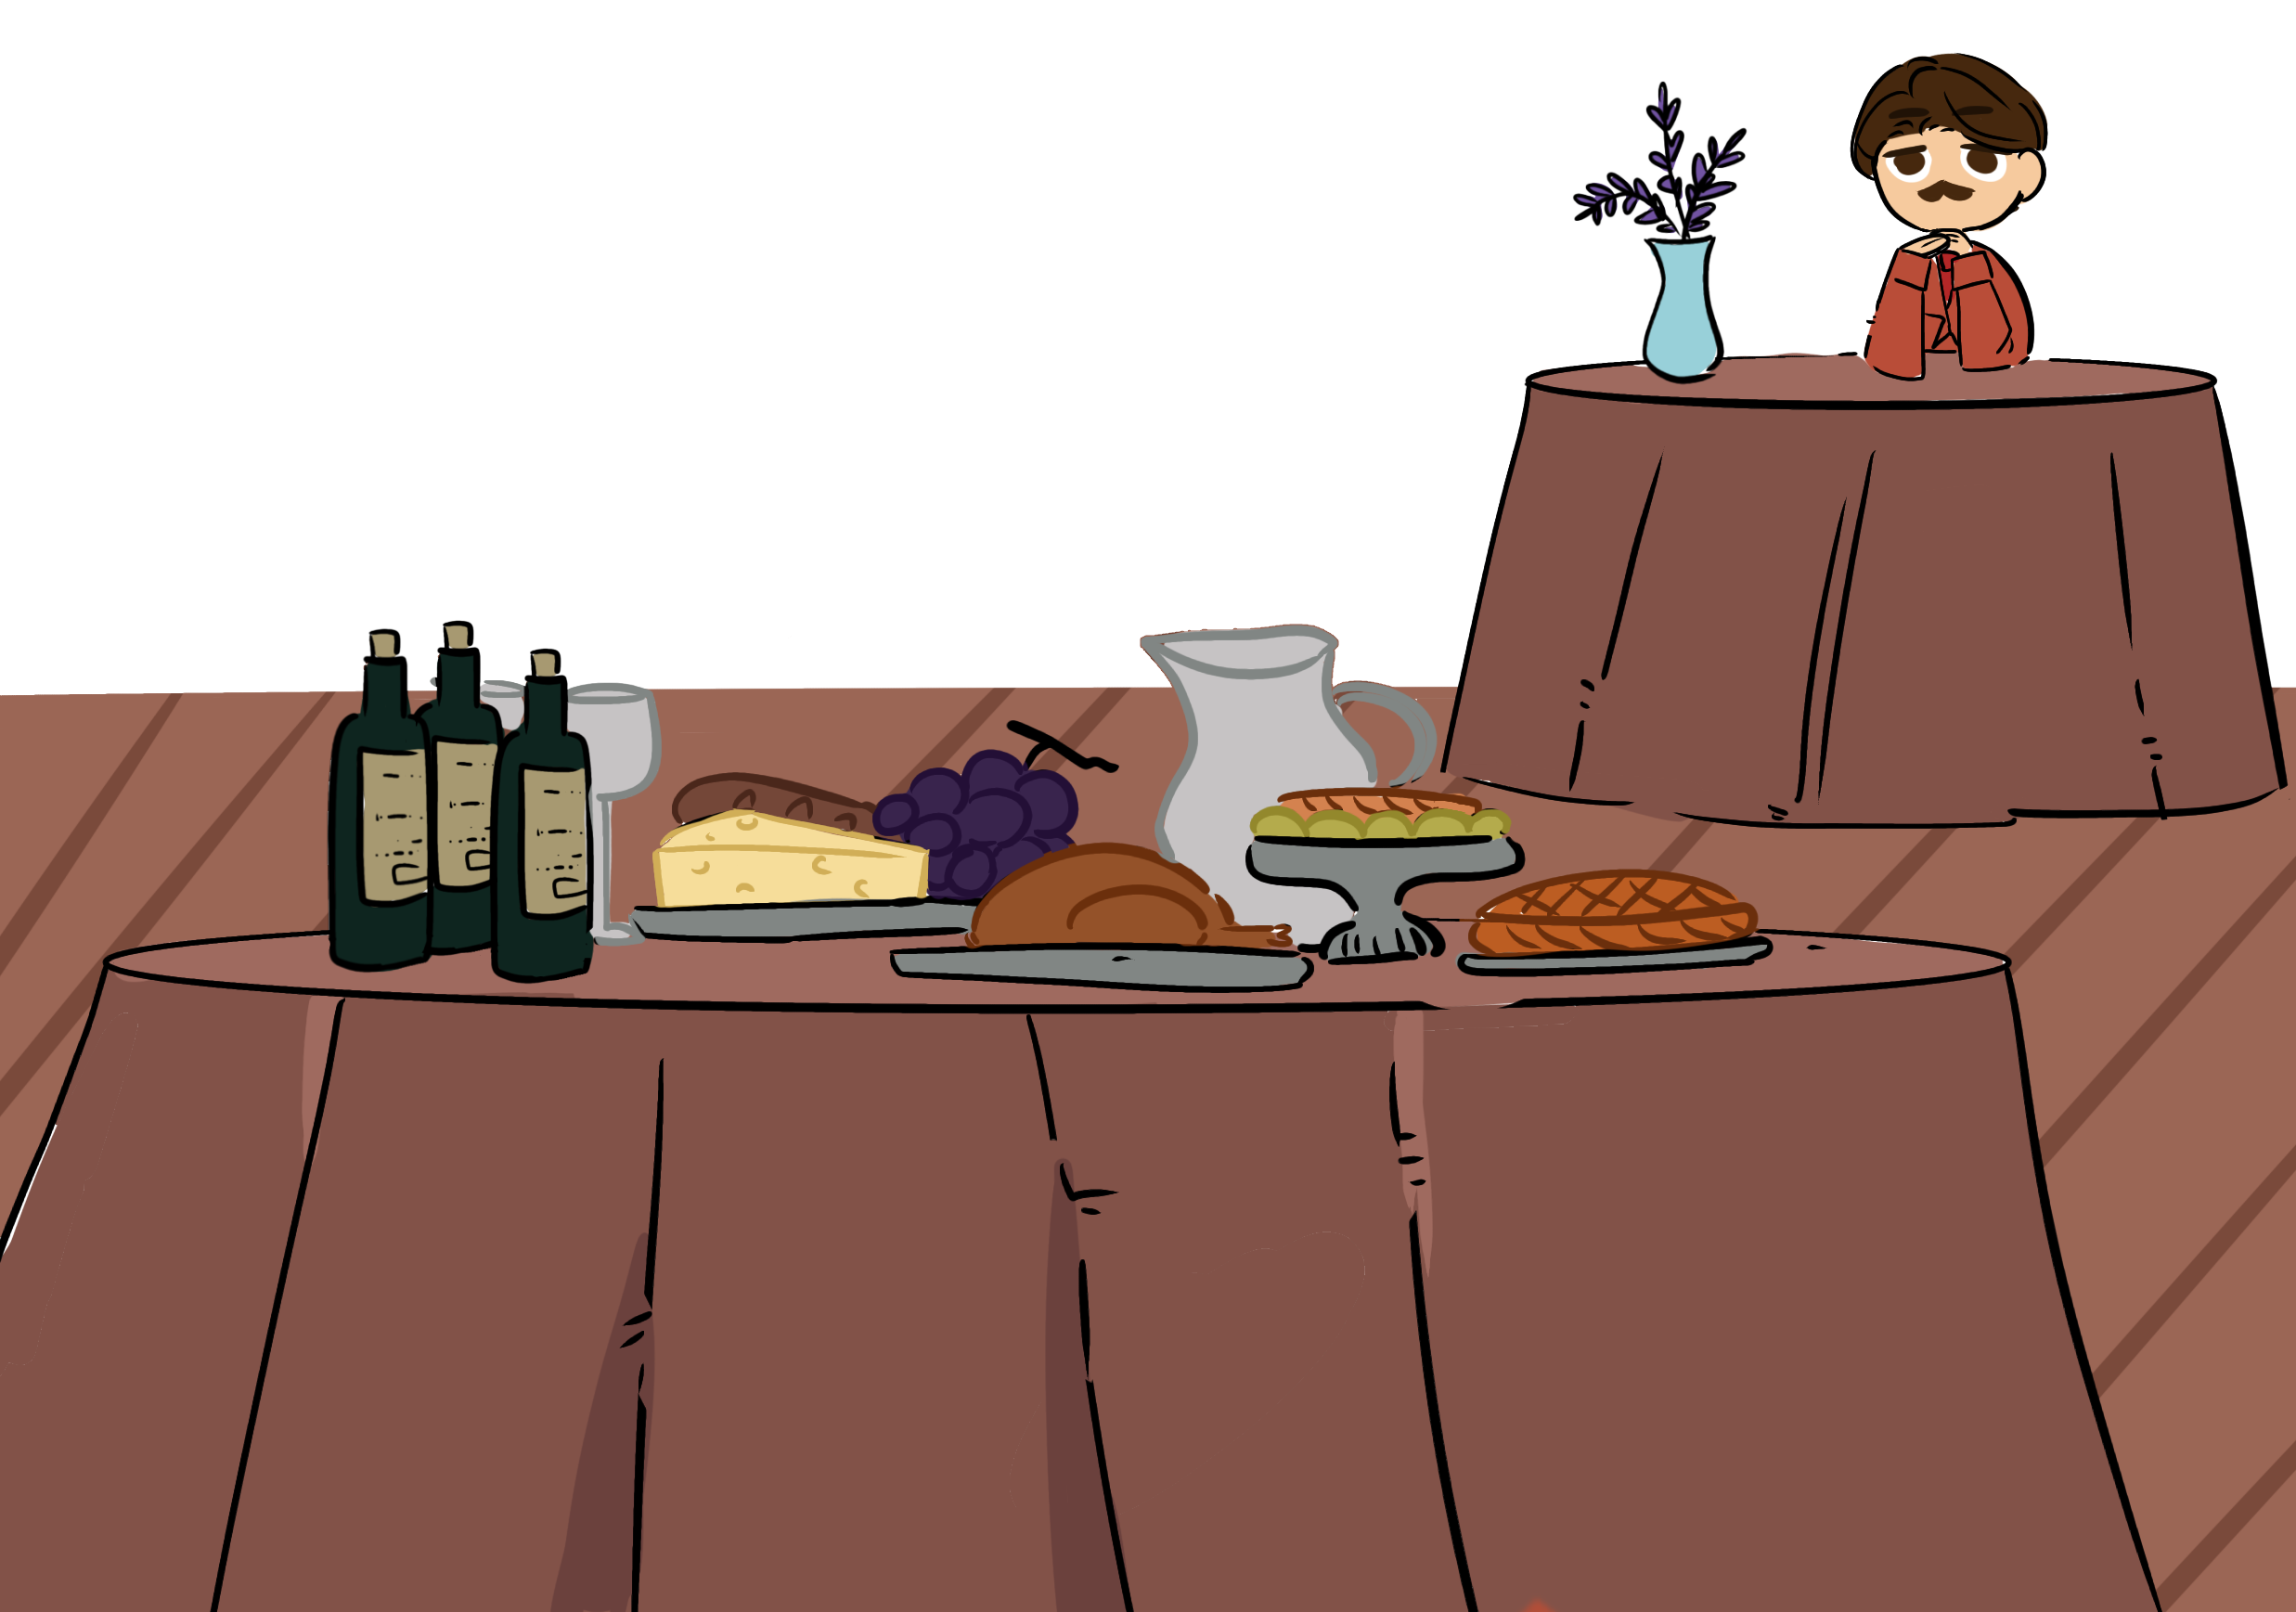
\includegraphics[width=1\linewidth]{xp}
%		\vspace*{-15pt}
%	\end{figure}
%%	Lời giải
%%	\vskip 0.1cm
%%	Ta nhận xét thấy rằng, không có hai người nào cùng đến từ trang trại Cừu Béo (ta gọi tắt là những người Cừu Béo, viết tắt là $C$) lại ngồi cạnh nhau, có nghĩa là bên cạnh mỗi người Cừu Béo luôn phải có hai người Bò Mập (viết tắt là $B$). Thật vậy, ta xét một chuỗi xích những người Cừu Béo ngồi cạnh nhau, vây xung quanh bởi những người Bò Mập. Người Cừu Béo ngồi ở rìa ngoài cùng sẽ có hai người ngồi cạnh - một là người Cừu Béo, một là người Bò Mập: điều này không thể xảy ra, vì khi đó thì người Cừu Béo đó hoá ra đã nói dối. Như vậy, không có hai người Cừu Béo nào ngồi cạnh nhau, và mỗi người Cừu Béo đều có hai người ngồi cạnh là những người Bò Mập.
%%	\vskip 0.1cm
%%	Ta sẽ gọi những người Bò Mập không bị nhầm lẫn là những người \textit{Bò Mập chân chính}. Theo điều kiện, hai người ngồi cạnh mỗi người Bò Mập phải đến từ các trang trại khác nhau. Như vậy, bên cạnh mỗi người Bò Mập phải luôn có một người Cừu Béo và một người Bò Mập. Điều này có nghĩa là chuỗi xích sau đây
%%	\begin{align*}
%%		BCBBCB\ldots BCB
%%	\end{align*}
%%	sẽ được lặp đi lặp lại cho đến khi gặp phải một người \textit{Bò Mập không chân chính}. Nếu trước người Bò Mập không chân chính này (tính theo chiều kim đồng hồ) có một người Cừu Béo, thì ngồi sau anh ta cũng phải là một người Cừu Béo khác. Còn nếu ngồi trước anh ta là một Bò Mập thì ngồi sau anh ta cũng phải là một người Bò Mập. Suy ra cách sắp chỗ ngồi với những Bò Mập không chân chính sẽ nhận được từ cách xếp ``$BCBBCB\ldots BCB$" hoặc bằng cách xếp một người Bò Mập không chân chính vào giữa hai Bò Mập, hoặc bằng cách cho một người Bò Mập chân chính đứng dậy ra khỏi bàn (khi đó một người Bò Mập ngồi cạnh anh ta sẽ biến thành một người Bò Mập không chân chính). Nếu thực hiện cách thứ nhất, số dư khi chia cho $3$ của tổng số người ngồi quanh bàn sẽ tăng thêm $1$. Còn nếu thực hiện cách thứ hai, số dư khi chia cho $3$ của tổng số người ngồi quanh bàn sẽ giảm đi $1$. Vì trong cách xếp ``$BCBBCB\ldots BCB$", số người ngồi quanh bàn chia hết cho $3$, còn số $25$ lại chia $3$ dư $1$, ta phải thực hiện hai lần cách thứ hai, bỏ đi hai người Bò Mập trong cách xếp gồm $27$ ghế theo quy luật ``$BCBBCB\ldots BCB$". Do đó, số người đến từ trang trại Bò Mập bằng
%%	\begin{align*}
%%		27\cdot \frac{2}{3}-2=16.
%%	\end{align*}
%%	Đáp số: Quanh bàn có $16$ người đến từ trang trại Bò Mập. 
%\end{multicols}
%\vspace*{-10pt}
%{\color{toancuabi}\rule{1\linewidth}{0.1pt}}
%\begingroup
%\AddToShipoutPicture*{\put(112,260){
\includegraphics[scale=1]{../tieude11.pdf}}} 
%\centering
%\endgroup
%\vspace*{50pt}
%
%\begin{multicols}{2}
%	$\pmb{1.}$ 	Ở tiệm bánh ngọt có bán hai loại bánh donut, loại to và loại bé.
%	\begin{figure}[H]
%			\centering
%			\vspace*{-5pt}
%			\captionsetup{labelformat= empty, justification=centering}
%			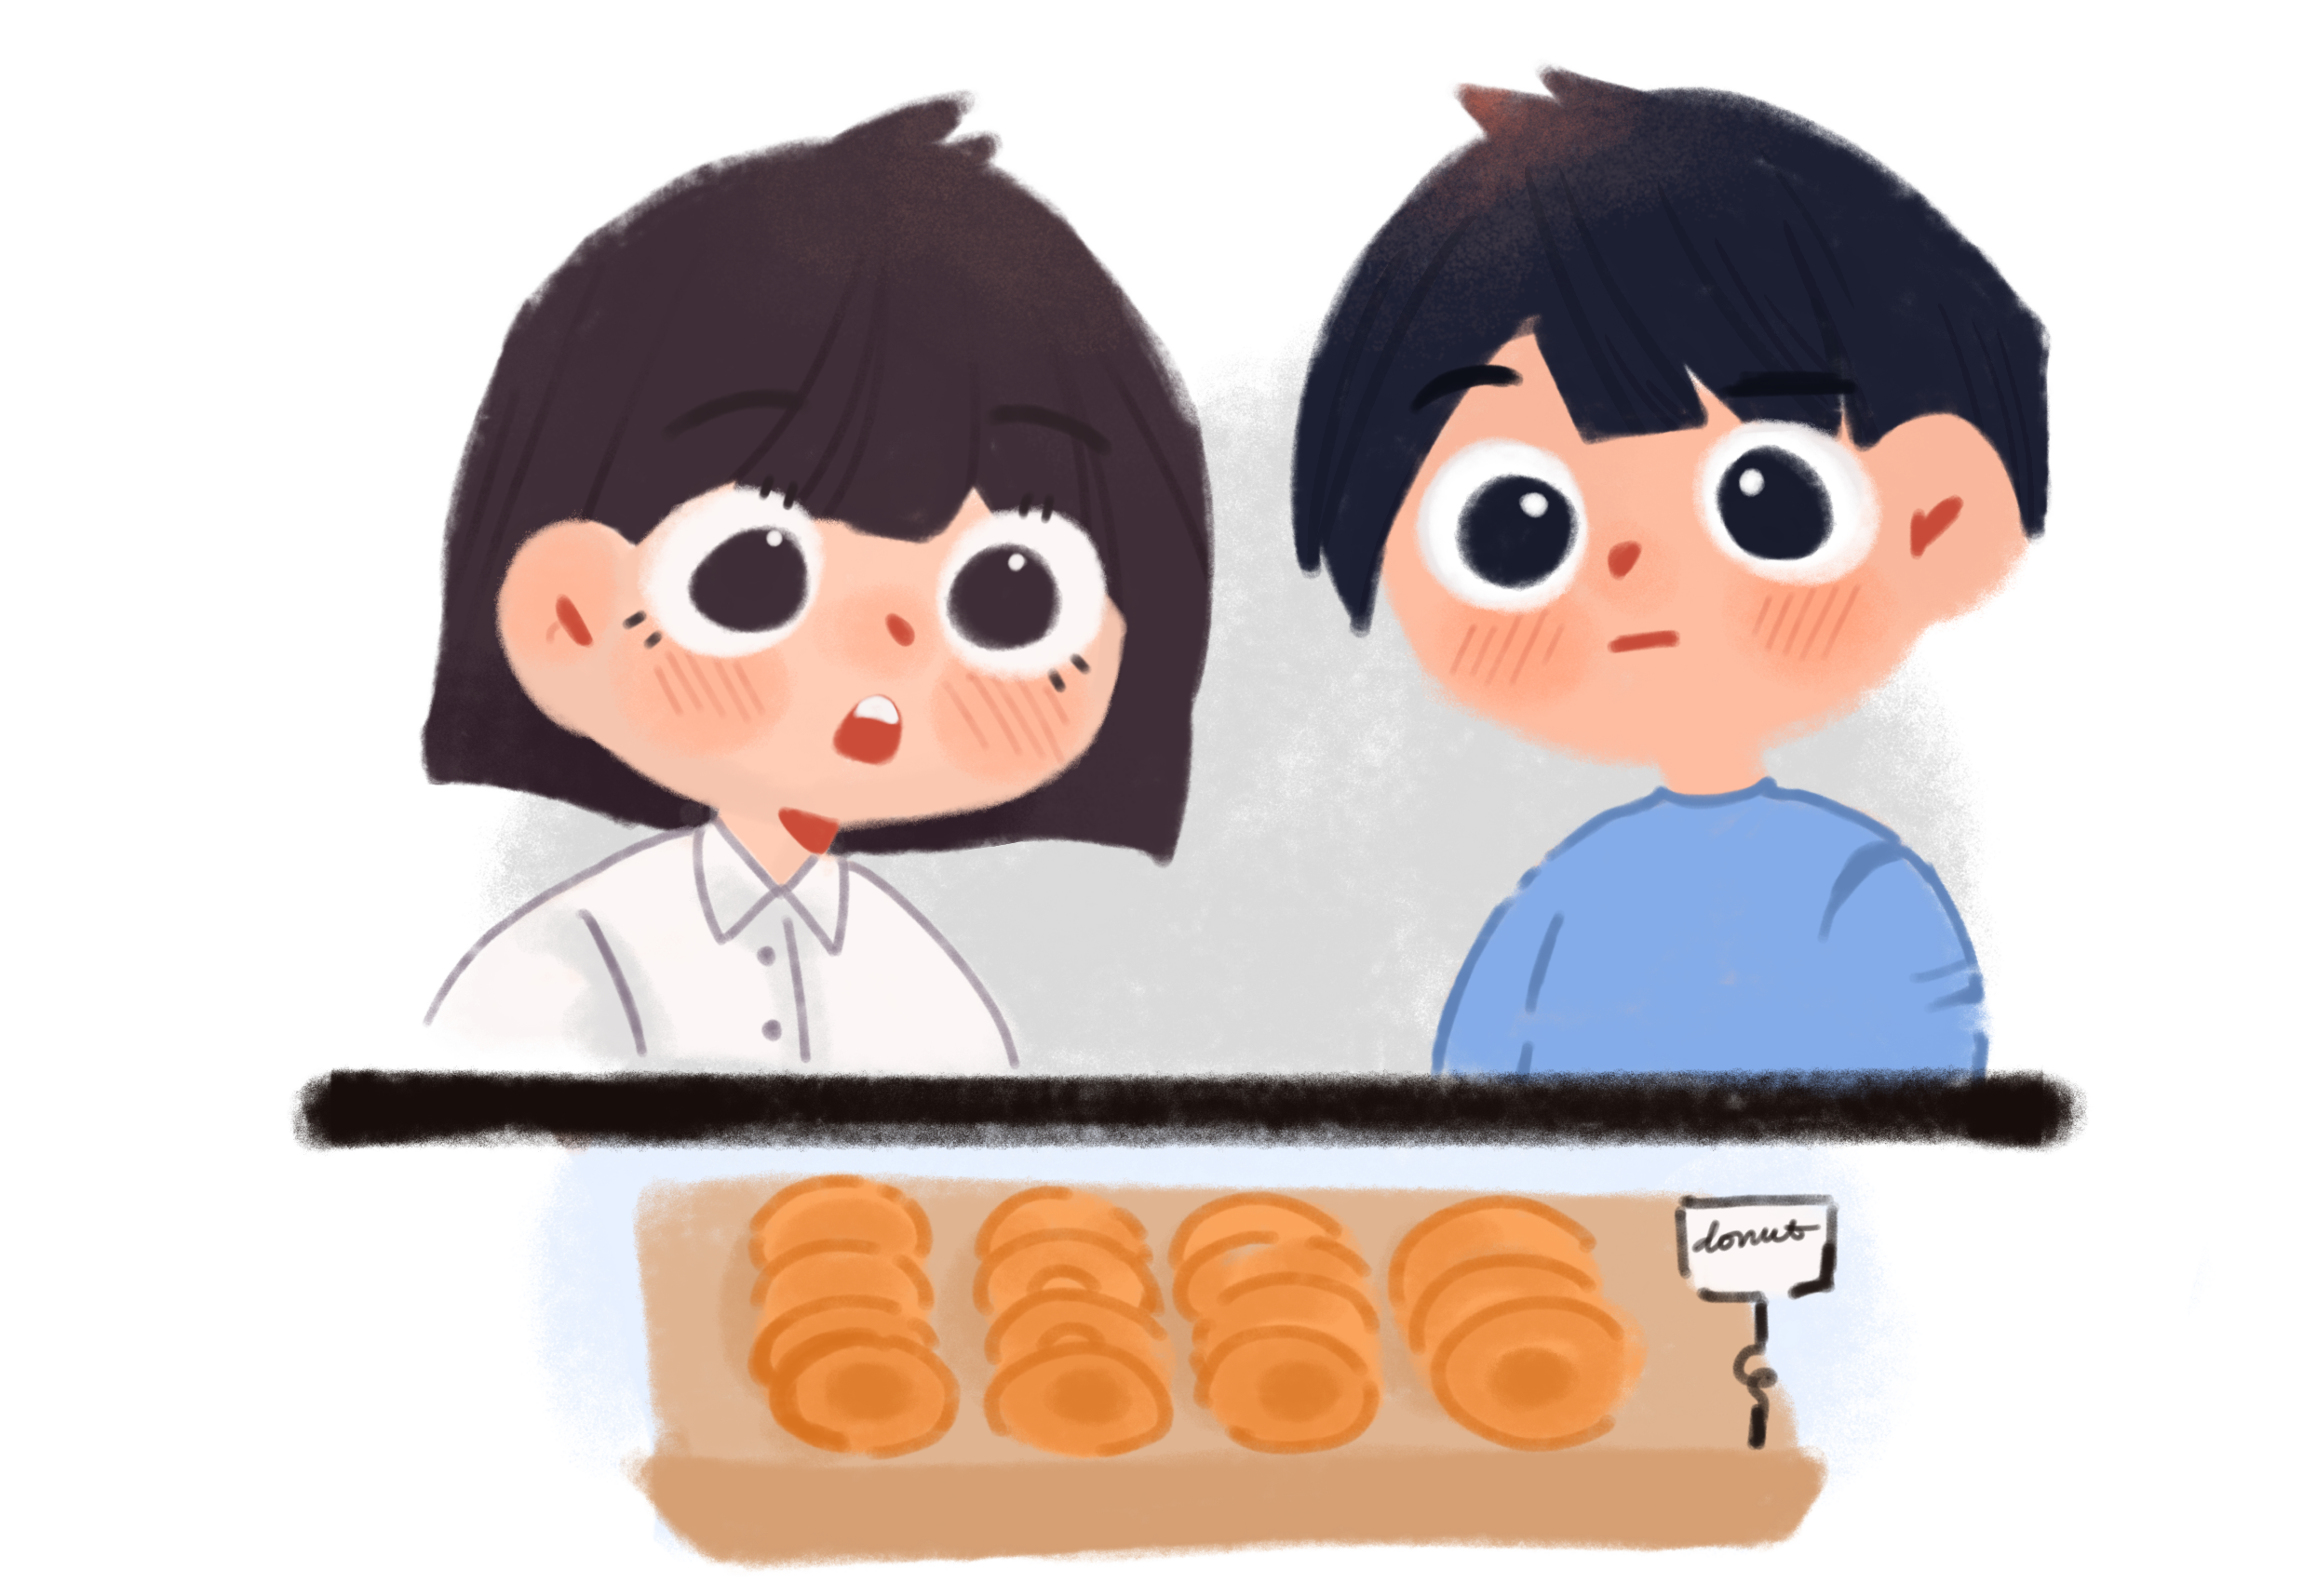
\includegraphics[width=1\linewidth]{H1}
%			\vspace*{-15pt}
%		\end{figure}
%	Loại donut to đắt gấp đôi loại donut bé. Hai bạn Hương và Bình cùng đến mua bánh donut, Hương mua $5$ chiếc donut loại to và $3$ chiếc loại bé, còn Bình mua $5$ chiếc loại bé và $3$ chiếc loại to. Hương phải trả nhiều hơn Bình là $20000$ đồng. Hỏi giá mỗi loại donut là bao nhiêu tiền?
%	\vskip 0.1cm
%	$\pmb{2.}$ 	Cậu bé Hùng và cô bé Lan học cùng một lớp. Trong lớp học của hai em, số học sinh nam nhiều gấp đôi số học sinh nữ. Hùng có số bạn nam học cùng lớp nhiều hơn số bạn nữ học cùng lớp là $7$ bạn. Hỏi Lan có bao nhiêu bạn nữ học cùng lớp?
%	\begin{figure}[H]
%			\centering
%			\vspace*{-5pt}
%			\captionsetup{labelformat= empty, justification=centering}
%			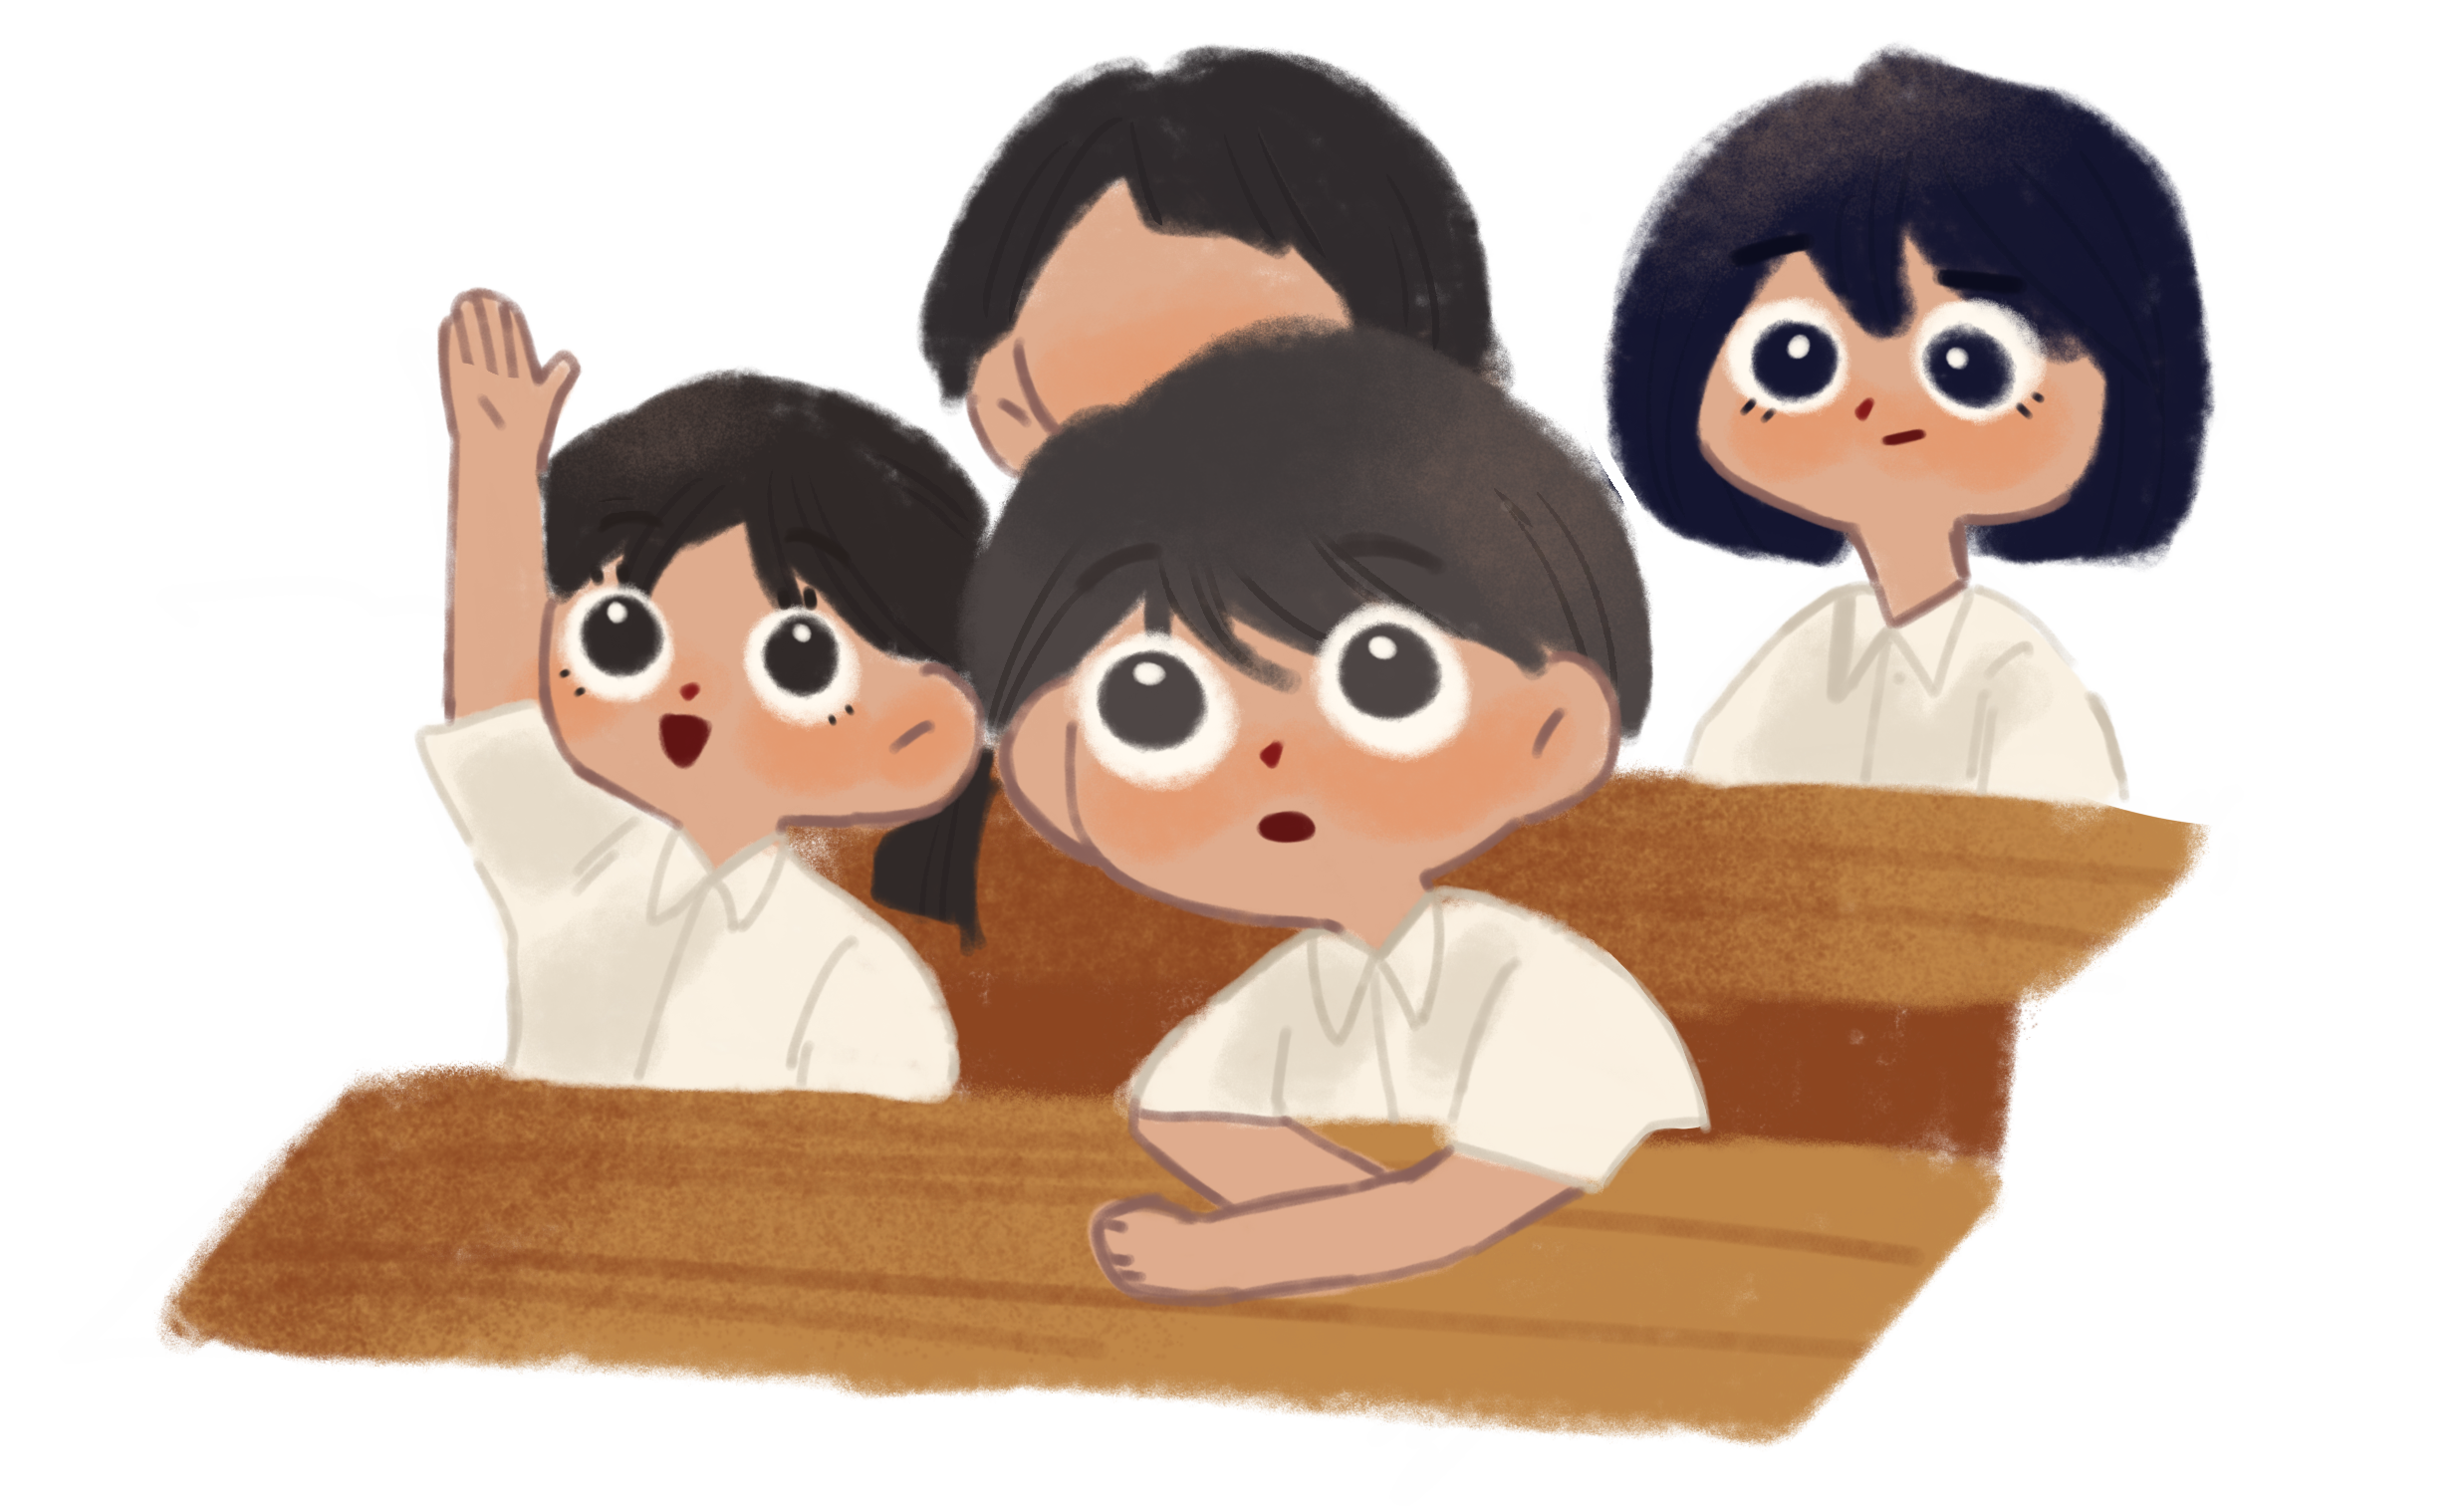
\includegraphics[width=1\linewidth]{H2}
%			\vspace*{-5pt}
%		\end{figure}
%	$\pmb{3.}$ 	Bé Tít được tặng một gói kẹo gồm kẹo sô--cô--la và kẹo caramel. Trong $10$ phút đầu tiên, Tít ăn hết $20\%$ số kẹo, hơn nữa có $25\%$ trong số đó là kẹo caramel. Tiếp theo Tít lại ăn thêm $3$ chiếc sô--cô--la, vì thế phần kẹo caramel trong số kẹo mà Tít đã ăn bị giảm xuống còn $20\%$. Hỏi trong túi kẹo ban đầu mà Tít được tặng có tất cả bao nhiêu chiếc kẹo?
%	\begin{figure}[H]
%			\centering
%			\vspace*{-5pt}
%			\captionsetup{labelformat= empty, justification=centering}
%			
\includegraphics[width=1\linewidth]{H3}
%			\vspace*{-15pt}
%		\end{figure}
%	$\pmb{4.}$ 	Có ba chú cáo là Bobby, Tommy và Ricky nói chuyện với nhau trên đồng cỏ. Tommy nói: ``Bobby không phải là chú cáo ranh mãnh nhất trong số chúng ta". Bobby nói: ``Tôi ranh mãnh hơn Tommy", Ricky nói: ``Bobby ranh mãnh hơn tôi". Biết rằng chú cáo ranh mãnh nhất trong ba chú nói dối, còn hai chú còn lại nói thật. Hỏi chú cáo ranh mãnh nhất tên là gì?
%	\begin{figure}[H]
%			\centering
%			\vspace*{-5pt}
%			\captionsetup{labelformat= empty, justification=centering}
%			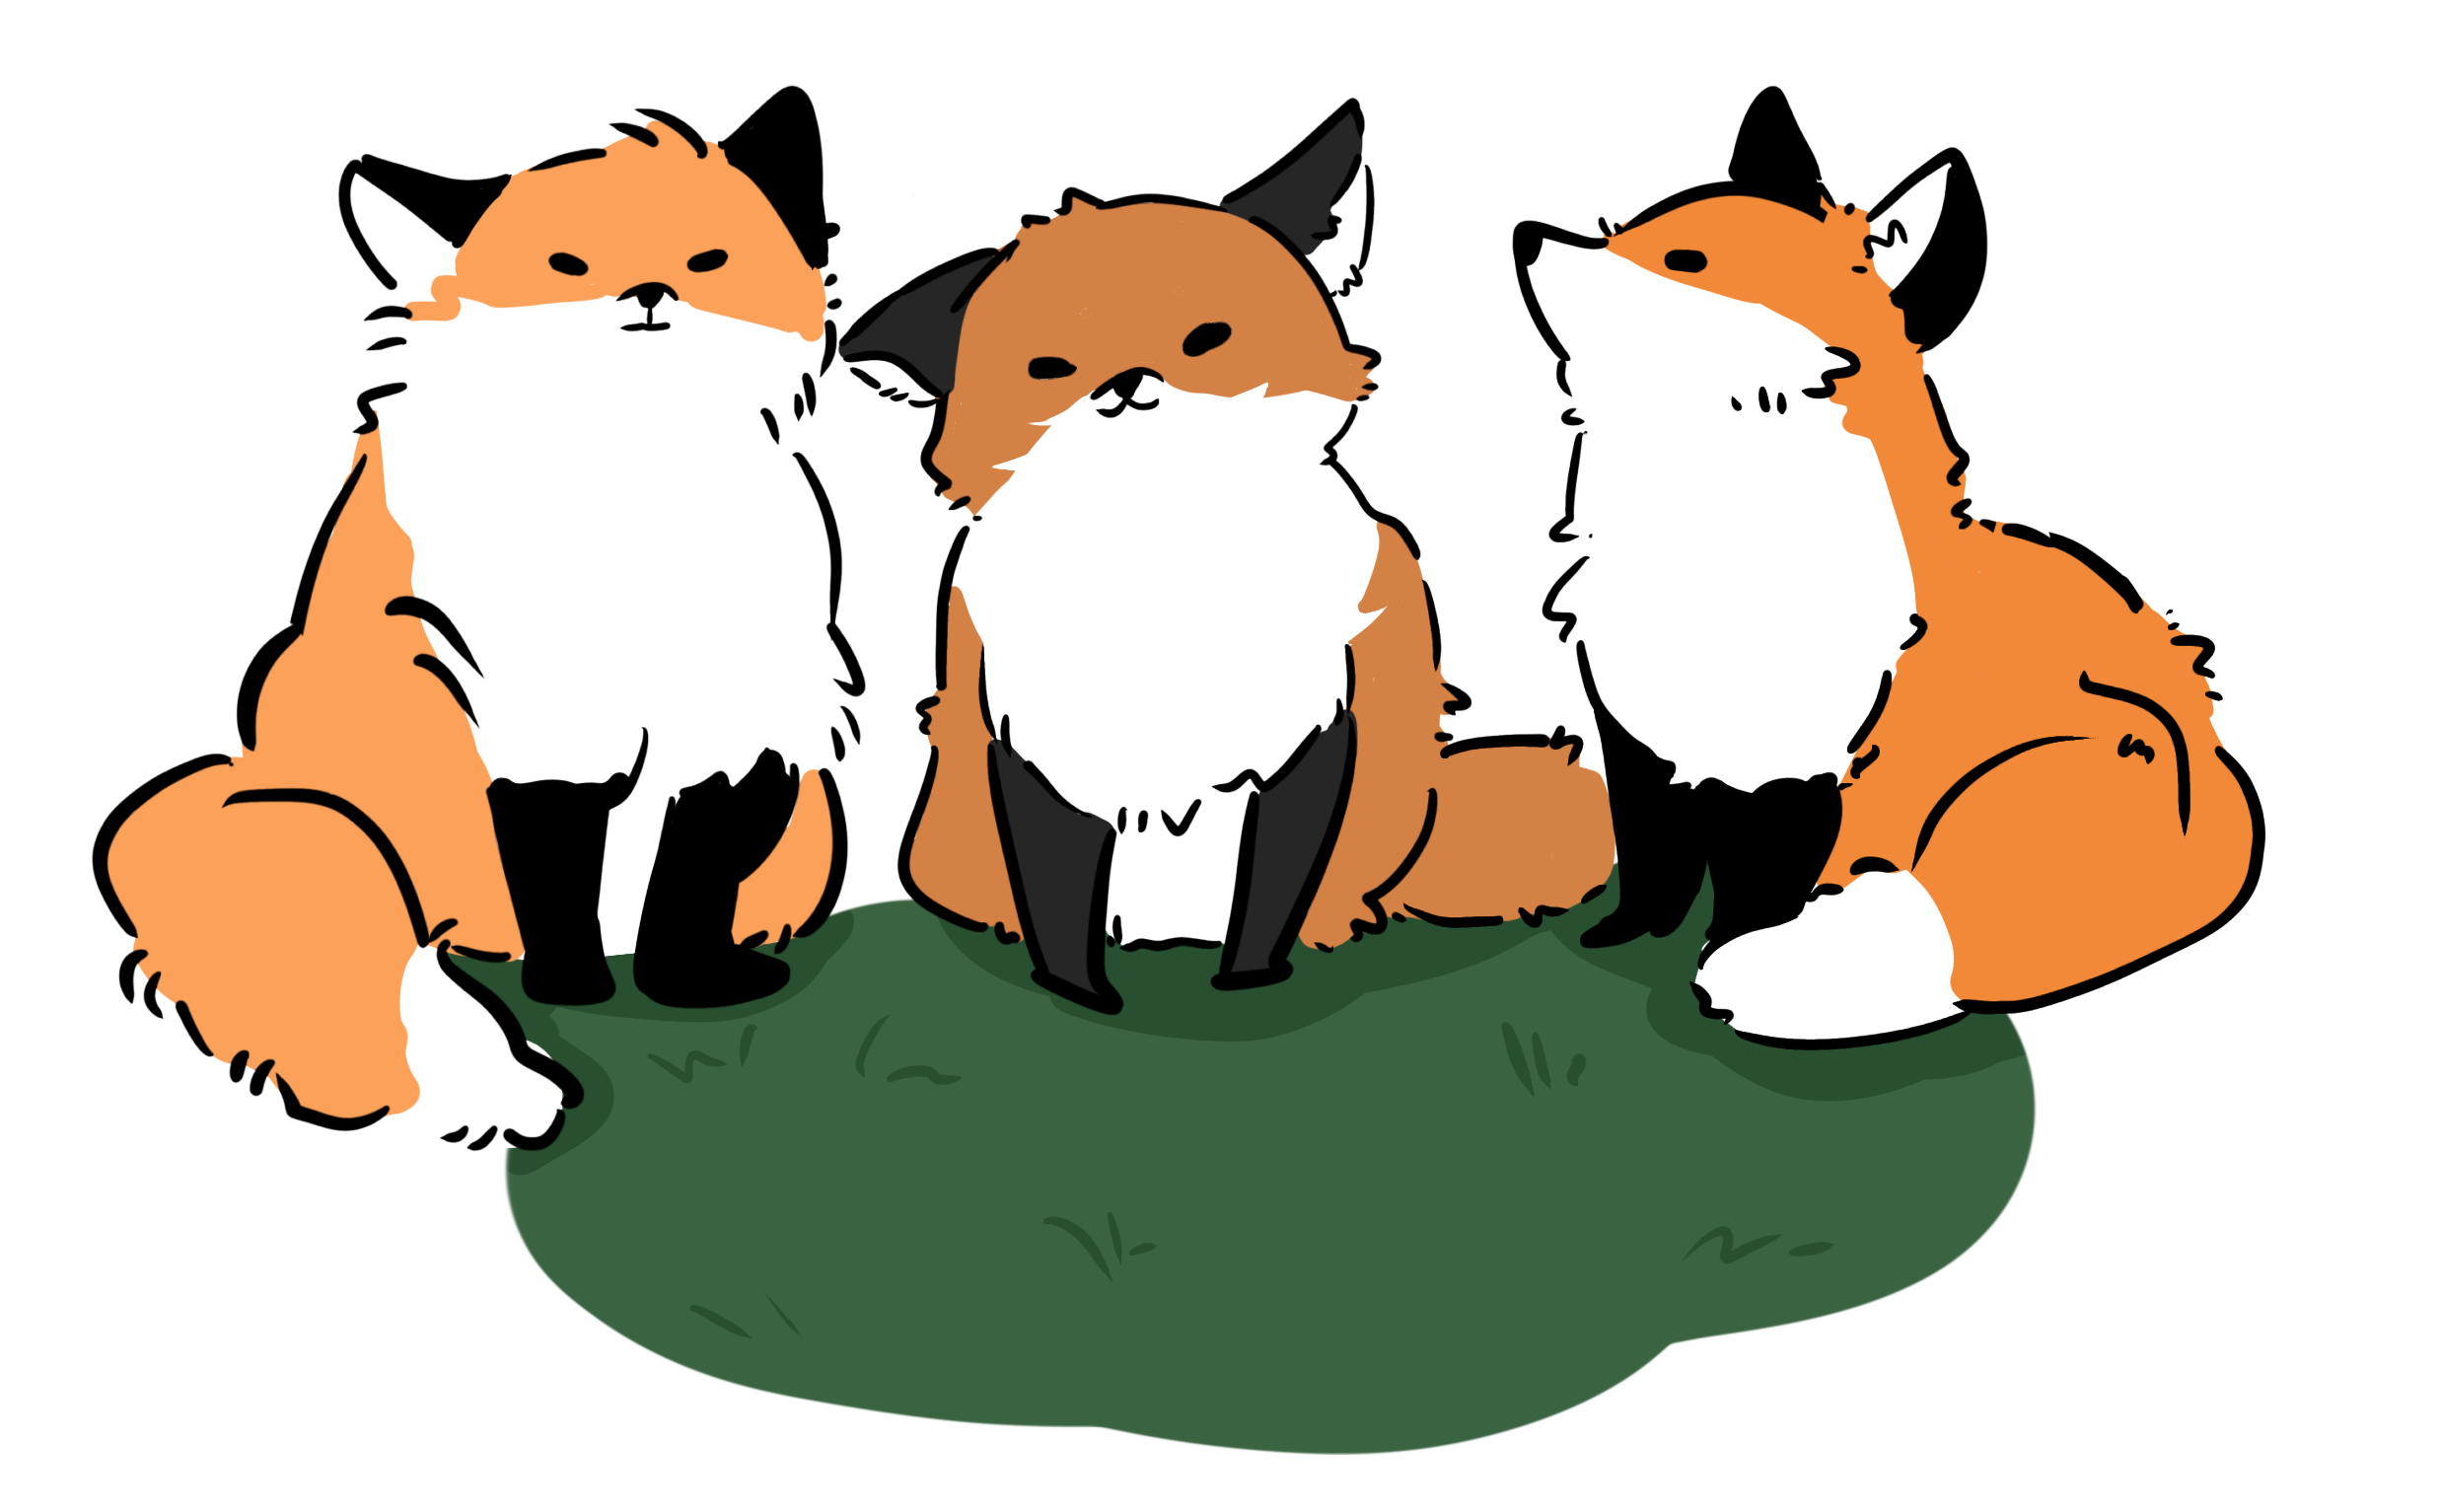
\includegraphics[width=0.8\linewidth]{H4}
%			\vspace*{-10pt}
%	\end{figure}
%	$\pmb{5.}$ 	Hai chiếc xe bus đi ngược chiều về phía nhau trên cùng một con đường với các vận tốc không đổi. Chiếc thứ nhất khởi hành từ Hà Nội lúc $11h$ sáng và tới Hạ Long vào lúc $16h$ chiều, chiếc thứ hai khởi hành từ Hạ Long lúc $12h$ trưa và đến Hà Nội lúc $17h$ chiều. Hỏi hai chiếc gặp nhau lúc mấy giờ?
%	\begin{figure}[H]
%			\centering
%			\vspace*{-5pt}
%			\captionsetup{labelformat= empty, justification=centering}
%			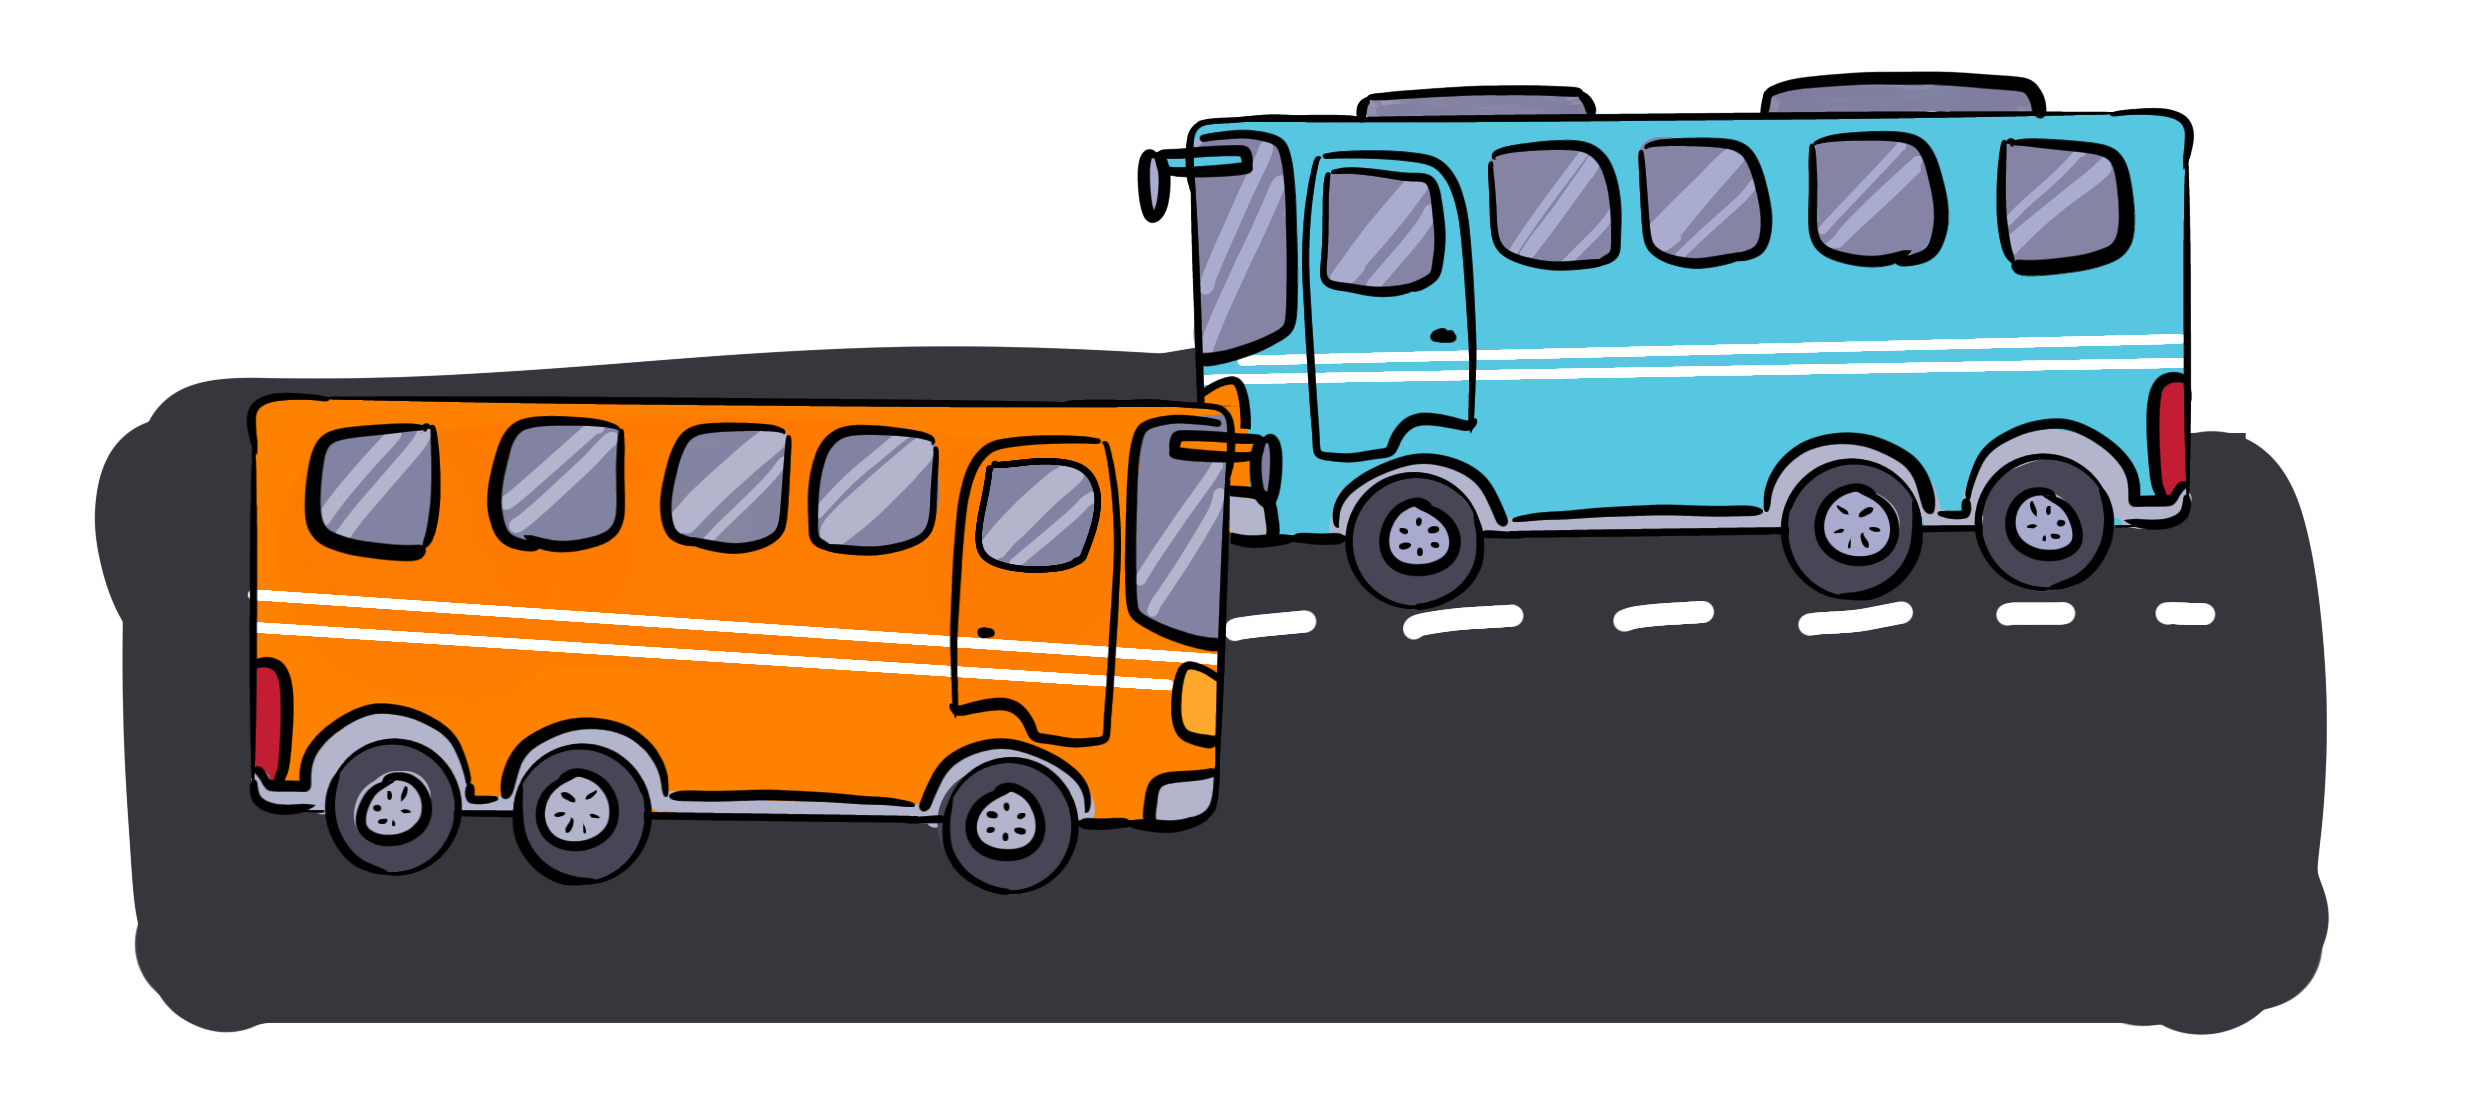
\includegraphics[width=1\linewidth]{H5}
%			\vspace*{-20pt}
%		\end{figure}
%	$\pmb{6.}$ Trên $6$ mặt của một con xúc xắc hình lập phương được ghi các số từ $1$ tới $6$ theo một cách nhất định. Người ta gieo con xúc xắc đó hai lần. Ở lần thứ nhất, tổng các số ở bốn mặt bên của xúc xắc bằng $12$, ở lần thứ hai tổng các số ở bốn mặt bên của xúc xắc bằng $15$. Hỏi số ở mặt đối diện với mặt được ghi số $3$ là số nào?
%	\begin{figure}[H]
%		\centering
%		\vspace*{-10pt}
%		\captionsetup{labelformat= empty, justification=centering}
%		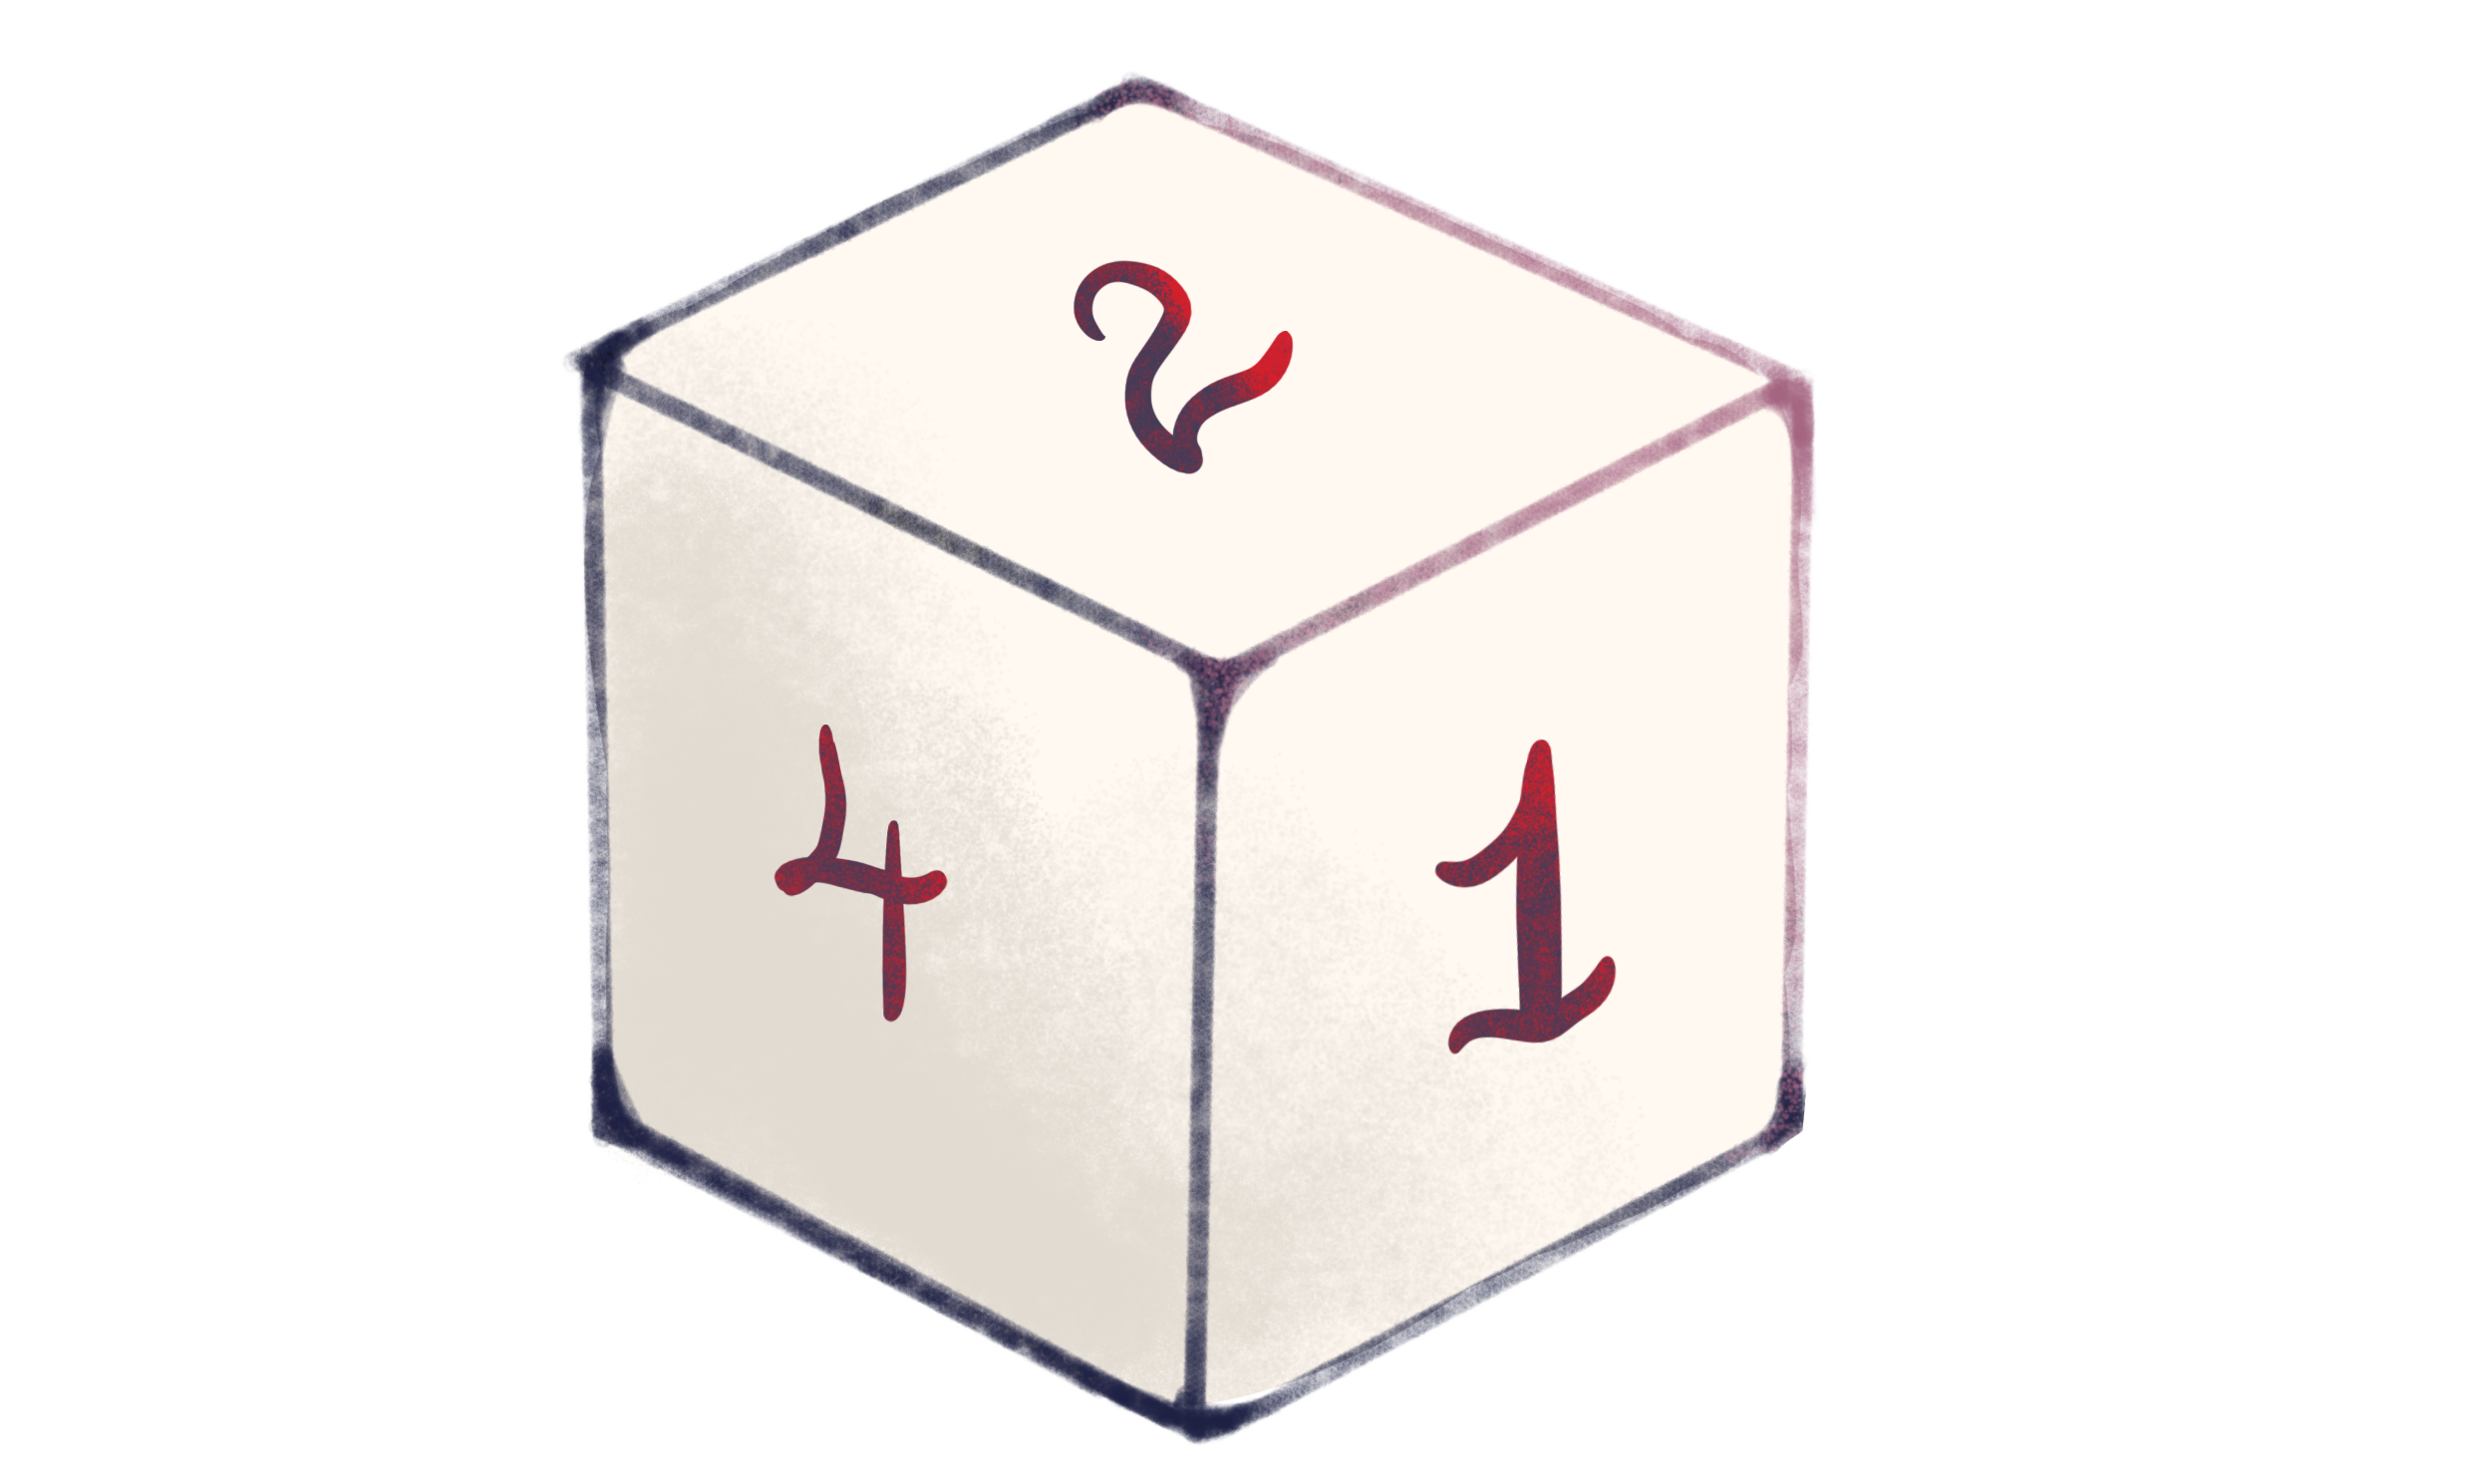
\includegraphics[width=0.85\linewidth]{H6}
%		\vspace*{-10pt}
%	\end{figure}
%	(Con xúc xắc có $6$ mặt, bao gồm $4$ mặt xung quanh, một mặt đáy và một mặt trên cùng).
%\end{multicols}
%\newpage
%\begingroup
%\AddToShipoutPicture*{\put(114,640){
\includegraphics[scale=1]{../tieude2.pdf}}} 
%\centering
%\endgroup
%\vspace*{75pt}
%
%\begin{multicols}{2}
%	$\pmb{1.}$ 	Trong ngày sinh nhật của mình, An mời $5$ người bạn tới nhà ăn bánh ga tô. An cắt cho người bạn thứ nhất $\dfrac{1}{6}$ chiếc bánh. Người bạn thứ hai được An cắt cho $\dfrac{1}{5}$ số bánh còn lại,
%	\begin{figure}[H]
%		\centering
%		\vspace*{-10pt}
%		\captionsetup{labelformat= empty, justification=centering}
%		
\includegraphics[width=0.6\linewidth]{Pi10_bai1}
%		\vspace*{-5pt}
%	\end{figure}
%	người bạn thứ ba được An cắt cho $\dfrac{1}{4}$ số bánh còn lại sau khi đã lấy bánh cho người bạn thứ hai, người thứ tư được chia $\dfrac{1}{3}$ số bánh còn lại sau khi đã lấy bánh cho người bạn thứ ba. Phần bánh cuối cùng được An cắt làm đôi và chia đều với người bạn thứ năm. Hỏi ai đã được chia nhiều bánh nhất?
%	\vskip 0.1cm
%	\textit{Lời giải.} Bạn nào cũng đã được chia số bánh đều như nhau (bằng $1/6$ chiếc bánh). Coi chiếc bánh ban đầu đã được chia thành $6$ phần bằng nhau, người bạn thứ nhất nhận $1$ phần, còn lại $5$ phần nên $1/5$ số bánh còn lại là $1$ phần bánh như người bạn đầu. Cứ như vậy, mỗi bạn đều nhận $1/6$ chiếc bánh ban đầu.
%	\vskip 0.1cm
%	$\pmb{2.}$ Tùng và Sơn cùng nhảy từ bờ xuống mặt nước và bơi về phía một hòn đảo.  Khi Sơn bơi được $40$ mét thì Tùng đã bơi đến được bờ của hòn đảo. Vừa chạm tới bờ, Tùng lại ngay lập tức bơi ngược lại và gặp lại Sơn vào thời điểm Sơn đã bơi thêm được $8$ mét nữa. Hỏi khoảng cách từ điểm xuất phát của hai bạn tới bờ hòn đảo là bao nhiêu?
%	\begin{figure}[H]
%		\centering
%		\vspace*{5pt}
%		\captionsetup{labelformat= empty, justification=centering}
%		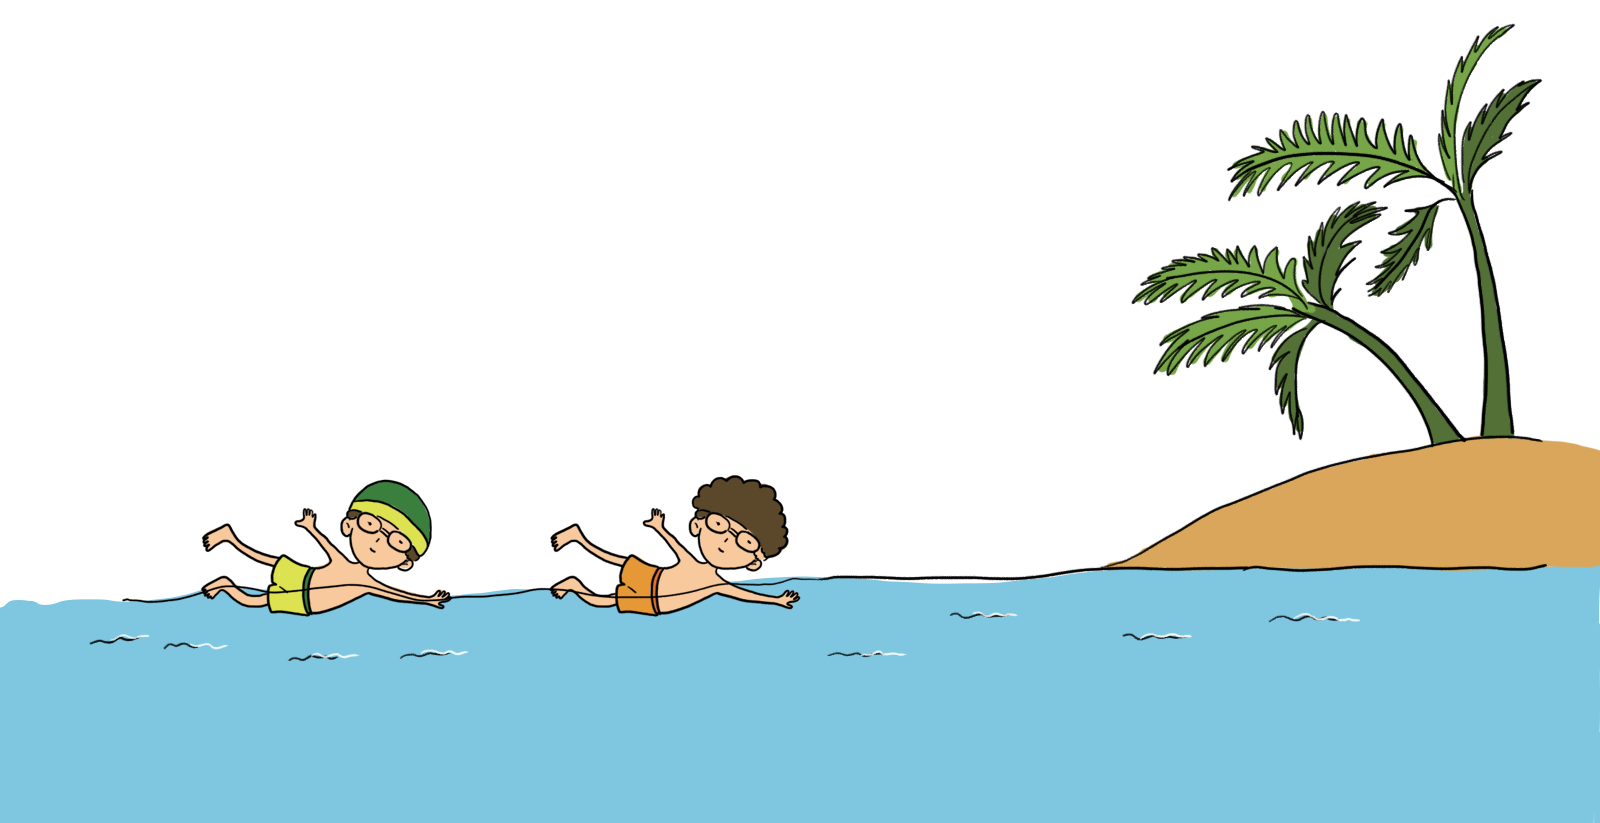
\includegraphics[width=1\linewidth]{Pi10_bai2}
%		\vspace*{-15pt}
%	\end{figure}
%	\textit{Lời giải.} 
%	Ký hiệu khoảng cách từ bờ tới bờ hòn đảo là $a$ mét. Do quãng đường $8$ mét bằng $1/5$ của khoảng cách $40$ mét, nên Tùng khi quay ngược lại đã bơi được $a/5$ mét trong số $(a-40)$ mét mà lúc đầu Sơn còn cách đảo. Do Sơn đã bơi thêm được $8$ mét cho tới khi gặp Tùng, nên
%	\begin{align*}
%		a/5+8=a-40.
%	\end{align*}
%	Suy ra $a=60$ (mét).
%	\vskip 0.1cm
%	\textit{Cách} $2$: Do quãng đường $8$ mét bằng $1/5$ của khoảng cách $40$ mét, và quãng đường bơi được của mỗi bạn tỷ lệ thuận với vận tốc bơi, nên quãng đường Tùng bơi được lúc xuôi gấp $5$ lần quãng đường bơi được lúc ngược lại đến khi gặp Sơn. Hiệu số của hai quãng đường là 
%	\begin{align*}
%		40+8=48 \text{ (mét)}
%	\end{align*}
%	Do đó quãng đường Tùng bơi lúc xuôi cũng là khoảng cách từ bờ tới bờ hòn đảo là
%	\begin{align*}
%		\frac{48}{5-1}\times 5 =60 \text{ (mét)}
%	\end{align*}
%	Đáp số: $60$ (mét).
%	\vskip 0.1cm
%	$\pmb{3.}$ Một tấm bìa hình chữ nhật kích thước $5\times 9$ được cắt ra thành $10$ hình chữ nhật nhỏ với các cạnh là các số nguyên. Em hãy chỉ ra rằng trong số các hình được cắt ra này có hai hình kích thước giống hệt nhau.
%	\begin{figure}[H]
%		\centering
%		\vspace*{-5pt}
%		\captionsetup{labelformat= empty, justification=centering}
%		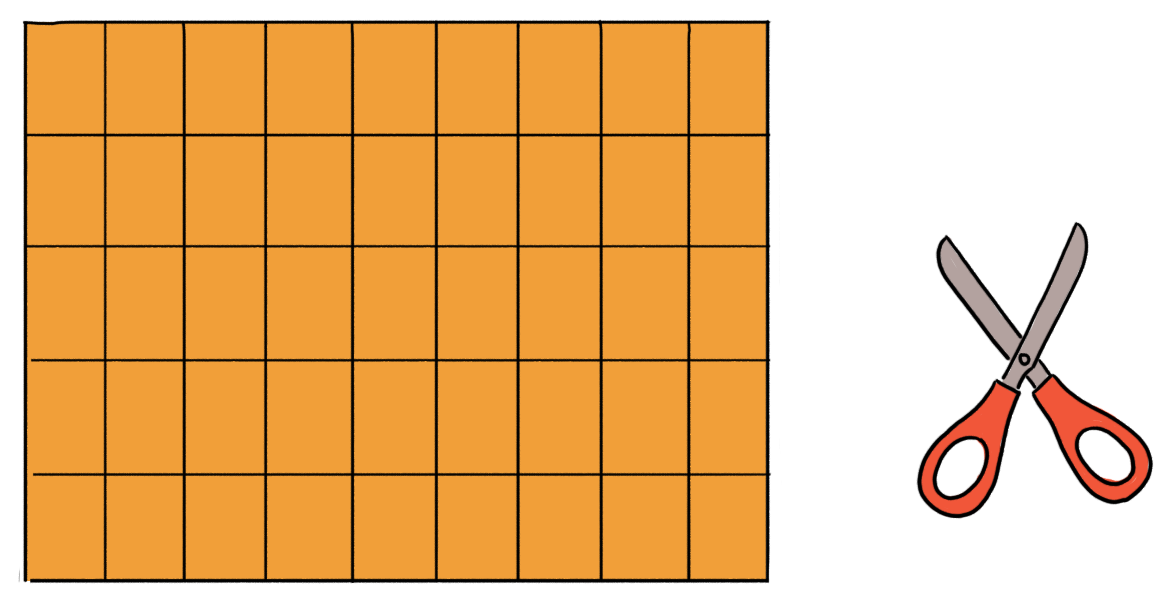
\includegraphics[width=1\linewidth]{Pi10_bai3}
%		\vspace*{-15pt}
%	\end{figure}
%	\textit{Lời giải.} Ta sẽ viết ra tất cả các hình chữ nhật có thể cắt ra được từ hình ban đầu mà các cạnh là các số nguyên theo thứ tự diện tích tăng dần:
%	\begin{align*}
%		&1 \times 1,1 \times 2,1 \times 3,1 \times 4,2 \times 2,1 \times 5,1 \times 6,\\
%		&2 \times 3,1 \times 7,1 \times 8,2 \times 4,\ldots
%	\end{align*}
%	Ta thấy tổng diện tích của $10$ hình khác nhau đầu tiên trong danh sách này là:
%	\begin{align*}
%		1+2+3+4+4+5+6+6+7+8 = 46
%	\end{align*}
%	Vậy tổng diện tích của $10$ hình khác nhau bất kỳ trong số chúng không nhỏ hơn $46$. Tuy nhiên diện tích của tấm bìa hình chữ nhật đã cho là 
%	\begin{align*}
%		5 \times 9 = 45
%	\end{align*}
%	Suy ra trong số $10$ hình được cắt ra từ tấm bìa đã cho có ít nhất hai hình kích thước giống hệt nhau.
%	\vskip 0.1cm
%	$\pmb{4.}$ Một nàng tiên đi tới một con suối nguồn với hai chiếc bình trên tay. Một chiếc bình có thể tích $5$ lít, còn chiếc kia có thể tích $4$ lít. Nước chảy ra từ suối nước theo hai dòng, một dòng mạnh hơn, còn dòng kia yếu hơn. Nàng tiên đặt đồng thời hai chiếc bình mỗi chiếc dưới một dòng nước.
%	\begin{figure}[H]
%		\centering
%		\vspace*{-5pt}
%		\captionsetup{labelformat= empty, justification=centering}
%		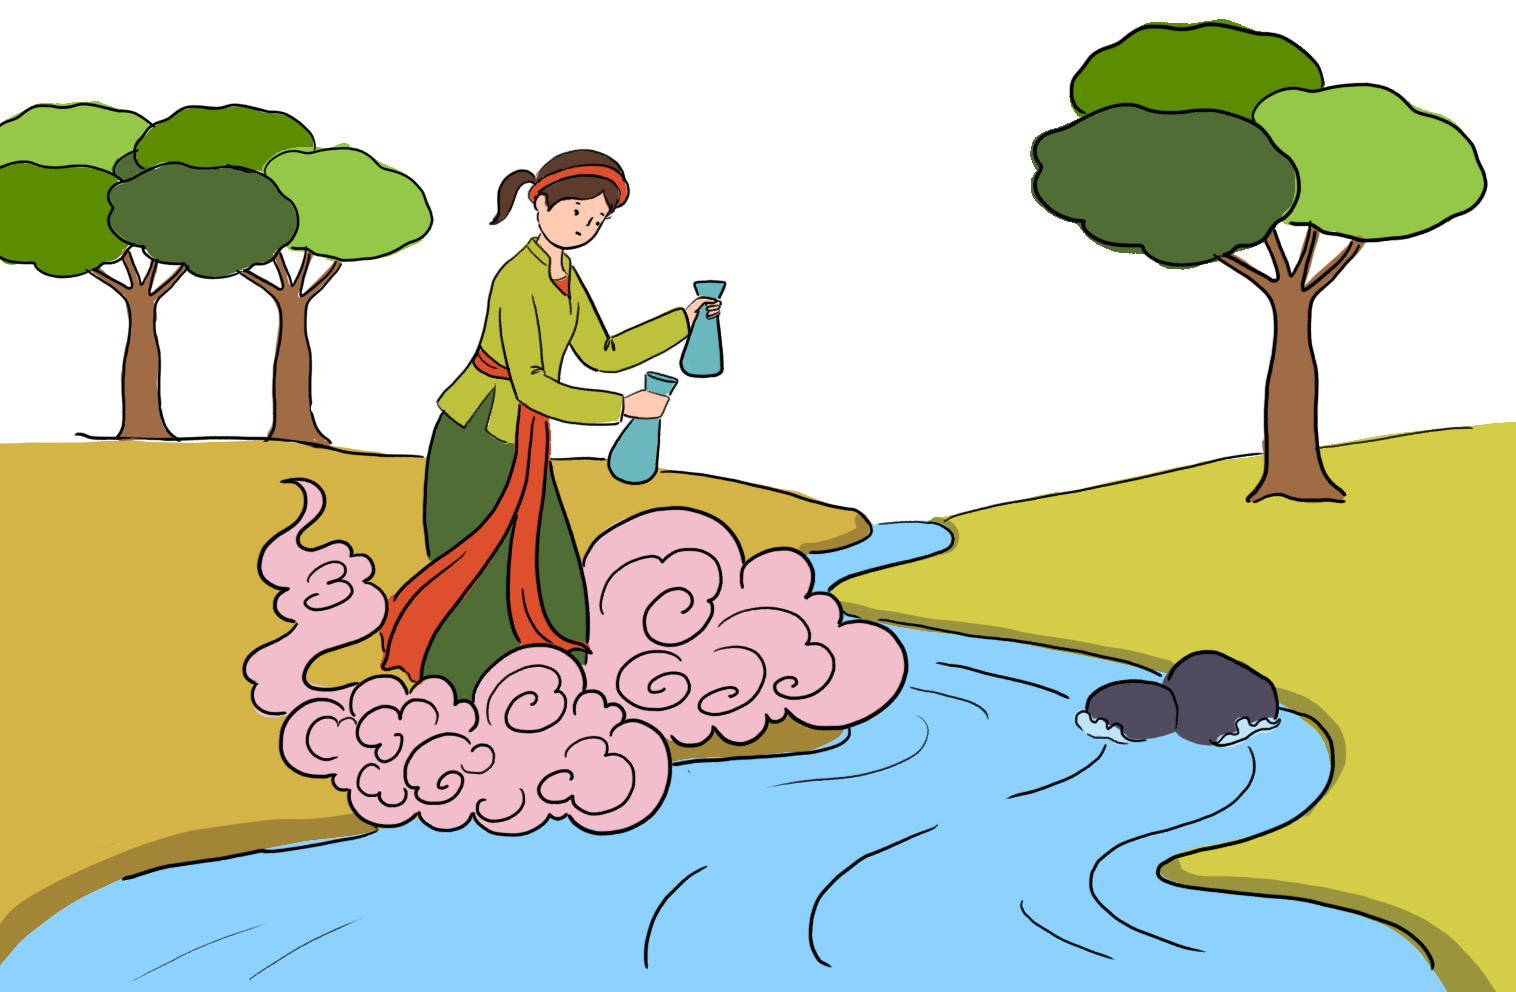
\includegraphics[width=1\linewidth]{Pi10_bai4}
%		\vspace*{-15pt}
%	\end{figure}
%	Khi đã hứng đầy được một nửa chiếc bình nhỏ, nàng tiên đổi vị trí hai bình cho nhau. Và vô cùng ngạc nhiên, hai chiếc bình được hứng đầy vào cùng một lúc. Hỏi  dòng nước mạnh chảy mạnh hơn gấp mấy lần so với dòng nước còn lại?
%	\vskip 0.1cm
%	\textit{Lời giải.} 	Giả sử dòng nước mà lúc đầu chiếc bình lớn hơn đã hứng chảy gấp $k$ lần so với dòng nước kia. Do trước khi đổi chỗ hai chiếc bình, trong bình nhỏ hơn đã hứng được $2$ lít, nên trong bình lớn hơn đã hứng được $2k$ (lít). Sau khi đổi chỗ, chiếc bình lớn đã hứng thêm được $5-2k$ (lít), còn chiếc bình nhỏ hứng được $2$ lít: số nước này gấp $k$ lần so với lượng nước chảy vào bình lớn sau khi đổi chỗ, tức là
%	\begin{align*}
%		k(5-2k)=2.
%	\end{align*}
%	Từ đây ta có $2k^2-5k+2=0$, suy ra $k=2$ hoặc $k=1/2$. Trong cả hai trường hợp ta luôn thấy một dòng nước chảy mạnh gấp đôi dòng còn lại.
%	 \vskip 0.1cm
%	$\pmb{5.}$ Bây giờ tuổi của Dũng đúng bằng gấp đôi tuổi của Hùng vào năm khi số tuổi của Dũng bằng tuổi của Hùng bây giờ. Khi Hùng có số tuổi bằng tuổi của Dũng bây giờ thì tổng số tuổi của hai người lúc đó sẽ bằng $63$. Hỏi bây giờ tuổi của Dũng và Hùng là bao nhiêu?
%	\vskip 0.1cm
%	\textit{Lời giải.} 	Gọi tuổi của Dũng bây giờ là $a$, còn tuổi của Hùng bây giờ là $b$. Khi đó điều kiện đầu tiên có thể viết thành hệ thức
%	\begin{align*}
%		a = 2(b-(a-b)),
%	\end{align*}
%	còn điều kiện thứ hai viết lại được ở dạng
%	\begin{align*}
%		a+(a+(a-b))=63. 
%	\end{align*}
%	Giản ước các hệ thức
%	\begin{align*}
%		&a = 2(b-(a-b))\\
%		&a+(a+(a-b))=63
%	\end{align*}
%	ta nhận được $3a=4b$ và $3a-b=63$. Suy ra $a=28,b=21$.
%	\vskip 0.1cm
%	Vậy bây giờ tôi $28$ tuổi và bạn $21$ tuổi.
%	\begin{figure}[H]
%		\centering
%		\vspace*{-5pt}
%		\captionsetup{labelformat= empty, justification=centering}
%		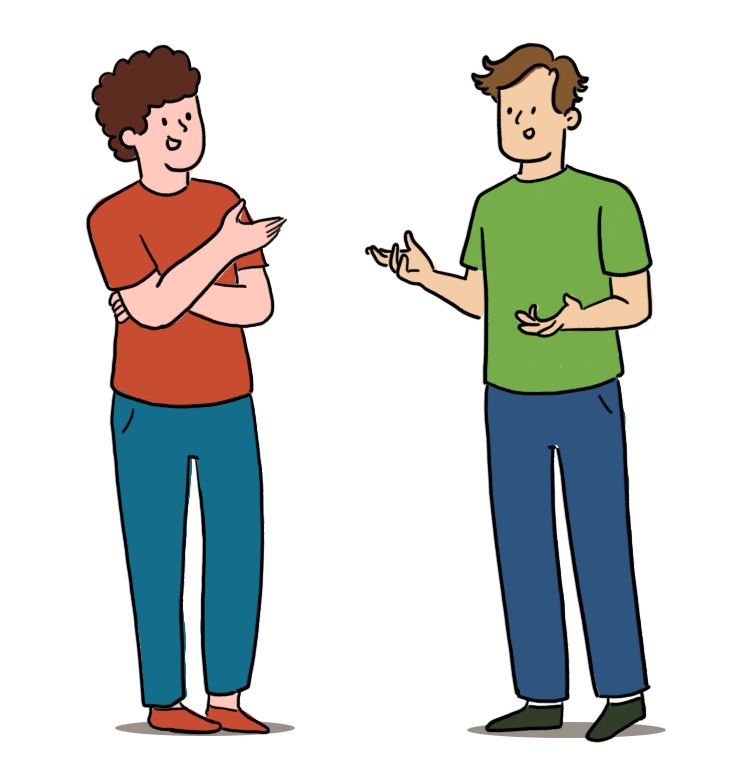
\includegraphics[width=0.75\linewidth]{Pi10_bai5}
%		\vspace*{-5pt}
%	\end{figure}
%	$\pmb{6.}$ Một chú kiến bò theo các cạnh của một hình  lập phương, chú chỉ quay đầu chuyển hướng tại các đỉnh của hình. Liệu có bao giờ xảy ra trường hợp khi chú đi qua một đỉnh nào đó của hình lập phương tận $25$ lần, trong khi chú chỉ đi qua tất cả các đỉnh còn lại tại mỗi đỉnh đúng $20$ lần?
%	\begin{figure}[H]
%		\centering
%		\vspace*{-5pt}
%		\captionsetup{labelformat= empty, justification=centering}
%		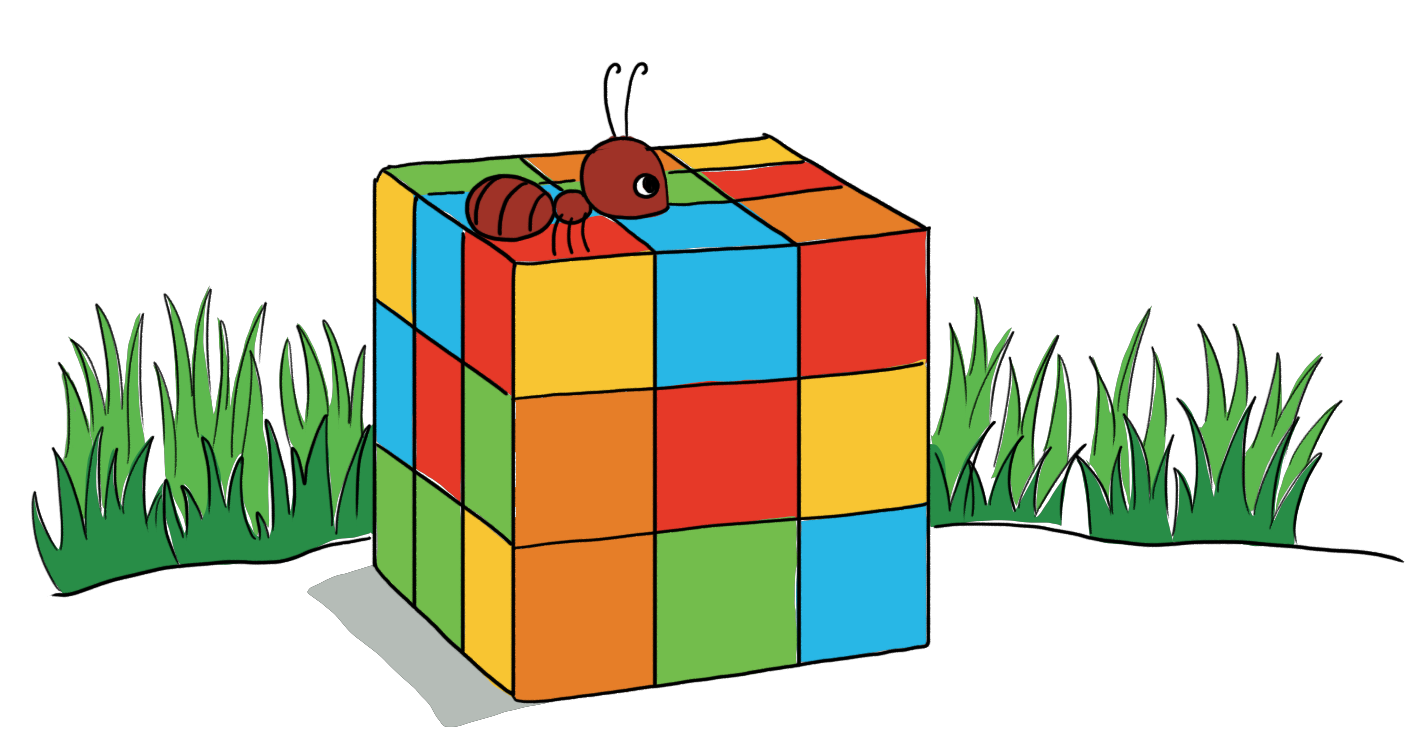
\includegraphics[width=1\linewidth]{Pi10_bai6}
%		\vspace*{-5pt}
%	\end{figure}
%	\textit{Lời giải.} 	Không thể xảy ra trường hợp nêu trong đề bài. Thật vậy, ta tô các đỉnh của hình lập phương bẳng hai màu xanh và đỏ như trong hình vẽ (hai đỉnh có chung cạnh là khác màu nhau). Khi đó theo mỗi đường di chuyển của chú kiến, các màu tại các đỉnh sẽ luân phiên xen kẽ nhau. Do đó tổng số lần đi qua các đỉnh màu đỏ của chú kiến khi bò theo các cạnh chỉ sai khác không quá $1$ so với tổng số lần đi qua các đỉnh màu xanh. 
%	\begin{figure}[H]
%		\centering
%		\vspace*{-5pt}
%		\captionsetup{labelformat= empty, justification=centering}
%		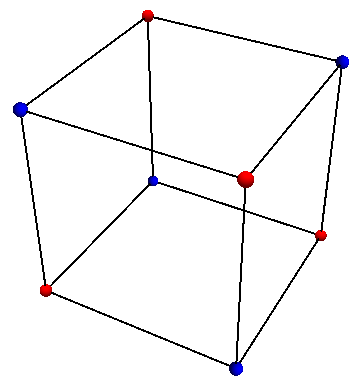
\includegraphics[width=0.6\linewidth]{b6}
%		\vspace*{-5pt}
%	\end{figure}
%	Tuy nhiên, trong trường hợp của đề bài, hiệu số lần đi qua $1$ đỉnh màu xanh và số lần đi qua $1$ đỉnh màu đỏ bằng $\pm5$ . Điều này mâu thuẫn.
%\end{multicols}
%%
%\newpage
%\thispagestyle{empty}
%\begingroup
%\blfootnote{$^1$\color{toancuabi}Theo https://www.idm314.org/2023-comic-challenge}
%\blfootnote{$^2$\color{toancuabi}Trường Đại Học Texas, Austin (TX), Hoa Kỳ}
%\AddToShipoutPicture*{\put(170,680){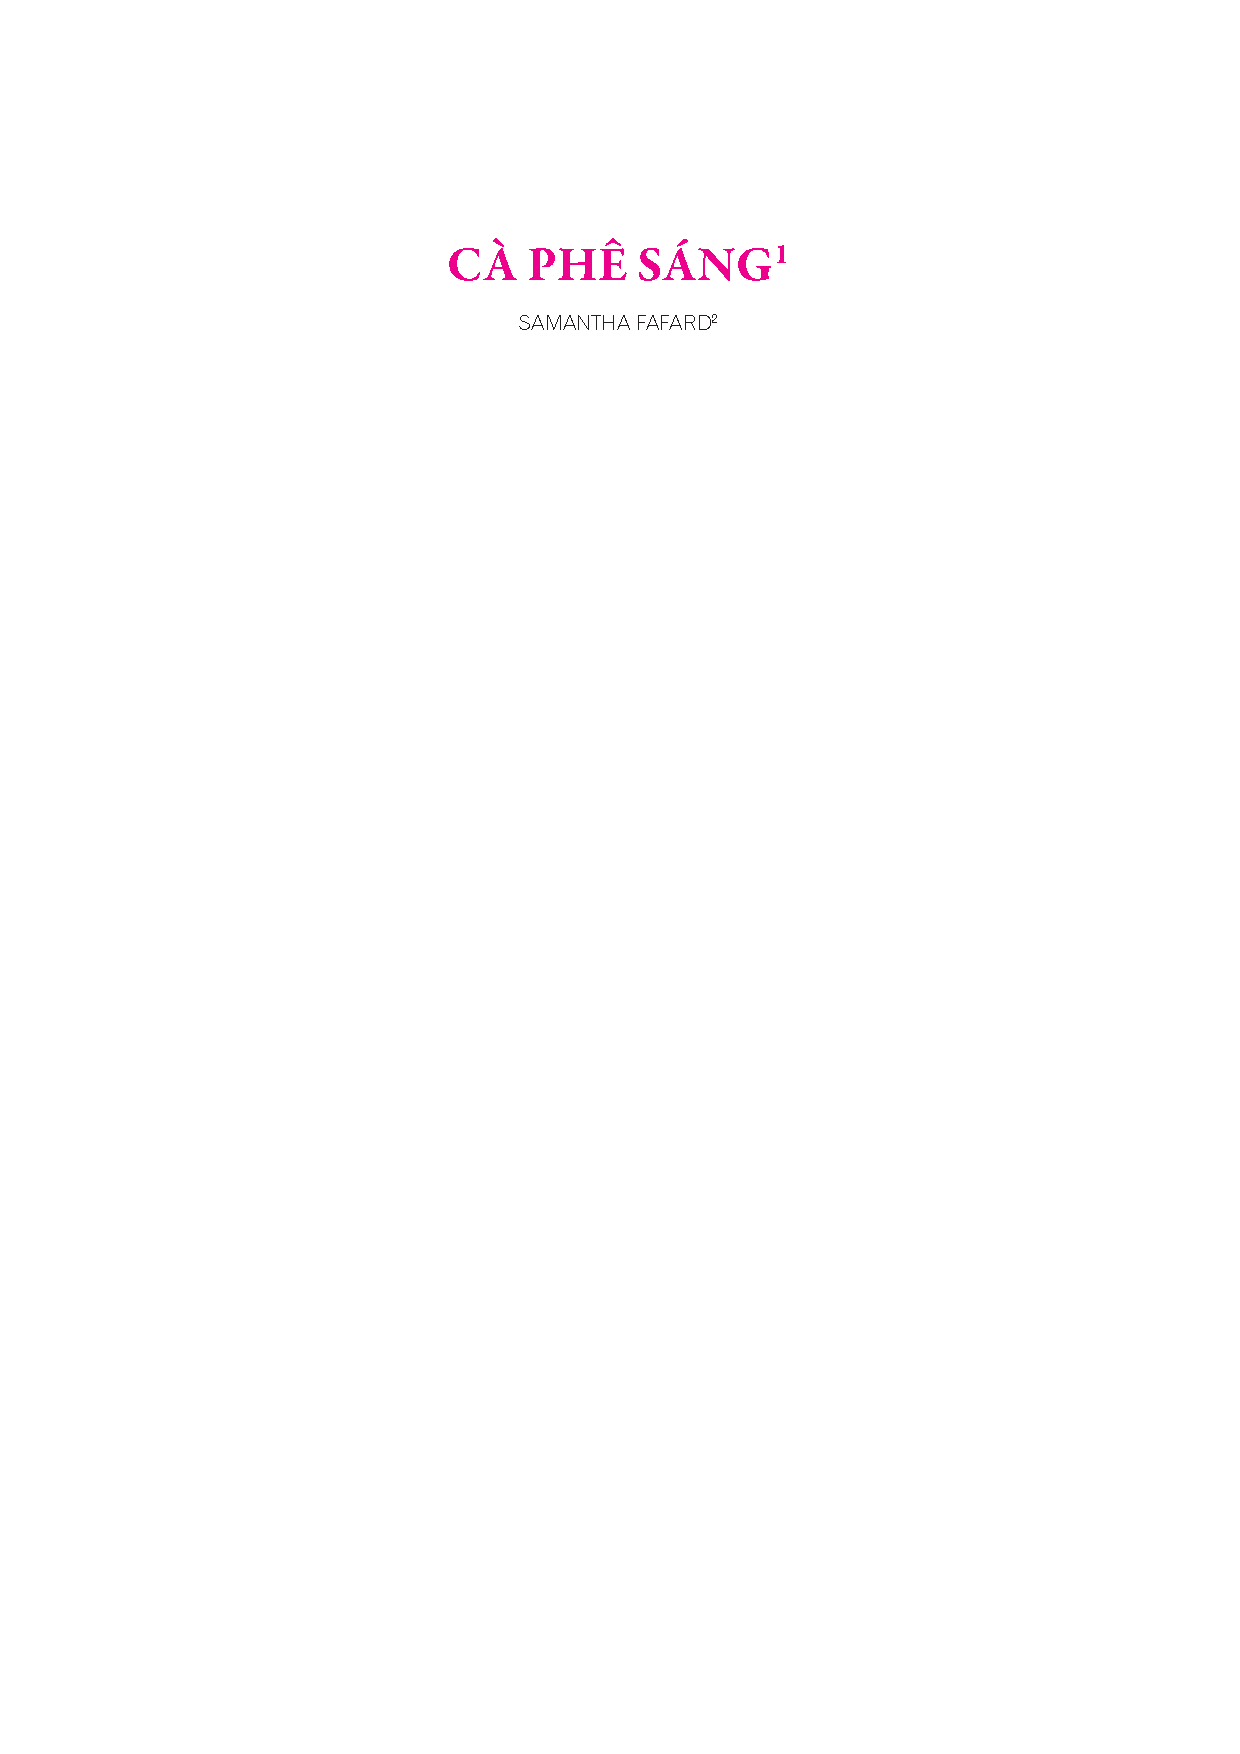
\includegraphics[scale=1]{../tieudehihi.pdf}}} 
%\centering
%\endgroup
%\vspace*{15pt}
%
%\begin{figure}[H]
%	\vspace*{5pt}
%	\centering
%	\captionsetup{labelformat= empty, justification=centering}
%	\includegraphics[width= 1\linewidth]{caphe}
%%	\caption{\small\textit{\color{}}}
%	\vspace*{-10pt}
%\end{figure}
%Các con dấu xếp hàng chờ cà phê để bắt đầu công việc của mình. Luôn phải chờ đợi theo thứ tự này. 
%
%\newpage
%\thispagestyle{empty}
%\begingroup
%\blfootnote{$^1$\color{toancuabi}Istituto comprensivo Silvio D'arzo settore tecnico grafico Reggio Emilia (Emilia Romagna, Italia Reggio, Emilia ), Italy.}
%\blfootnote{$^2$\color{toancuabi}Stadium là đơn vị độ dài, bằng độ dài một sân vận động thời Hy Lạp--La Mã, vào khoảng $156$ mét.}
%\AddToShipoutPicture*{\put(126,650){\includegraphics[scale=1]{../tieudehihi2.pdf}}} 
%\centering
%\endgroup
%\vspace*{50pt}
%
%\begin{figure}[H]
%	\vspace*{5pt}
%	\centering
%	\captionsetup{labelformat= empty, justification=centering}
%	\includegraphics[width= 0.75\linewidth]{320}
%	%	\caption{\small\textit{\color{}}}
%	\vspace*{-10pt}
%\end{figure}
%Khoảng cách giữa Siena và Alexandria là $5000$ stadium$^2$  và vào giữa ngày hạ chí ở Siena, mặt trời chiếu vuông góc với trái đất trong khi ở Alexandria nó nghiêng $7{,}2^\circ$. Do đó ông đã tính chu vi Trái Đất xuống tương đương $7{,}2:360=5000:x$.
\newpage
\graphicspath{{../toancuabi/toantienganh/}}
\begingroup
\thispagestyle{toancuabinone}
\blfootnote{$^1$\color{toancuabi}Ottawa, Canada.}
\AddToShipoutPicture*{\put(60,733){\includegraphics[width=17.2cm]{../mathc.pdf}}}
%\AddToShipoutPicture*{\put(-2,733){\includegraphics[width=17.2cm]{../mathl.pdf}}} 
\AddToShipoutPicture*{\put(66,670){\includegraphics[scale=1]{../tieudeb.pdf}}} 
\centering
\endgroup
\vspace*{40pt}

\begin{multicols}{2}
	This article is the second part of the series on demonstration \textit{Proof by Contradiction}.
	\vskip 0.2cm
	\PIbox{
	\textbf{\color{toancuabi}Example $\pmb6$.}
	Twenty--five persons from $8$ different provinces elected to the National Congress.
	Prove that at least $4$ of them are from the same province.}
	\vskip 0.2cm
	\textit{Solution.}
	Assume that this is not true. Then no $4$ of them are from the same province.
	In this case, not more than $3$ persons are from the $1^{\text{st}}$ province, not more than $3$ from the $2^{\text{nd}}$, and so on.
	Altogether, there are not more than $3 \times 8 = 24$ persons. This contradicts the fact that there are $25$ persons.
	\vskip 0.2cm
	\PIbox{\textbf{\color{toancuabi}Example $\pmb7$.}
	At the graduation event of the School of Wizardry, $5$ outstanding students called to the podium.
	They standing in a row. Altogether, these $5$ students know $300$ different spells.
	Prove that there are $2$ students standing next to each other who, if combined, know at least $100$ spells.}
	\vskip 0.1cm
	\textit{Solution.}
	Suppose that this is not true. Then the $1^{\text{st}}$ and $2^{\text{nd}}$ students together know less than $100$ spells,
	and the $4^{\text{th}}$ and $5^{\text{th}}$ students together know less than $100$ spells.
	Then these four know less than $200$ spells together. In this case, the $3^{\text{rd}}$ student knows more than $100$ spells.
	\vskip 0.2cm
	\PIbox{\textbf{\color{toancuabi}Example $\pmb8$.}
	The only way to travel in the Kingdom of so many swamps is to use magic carpets.
		Twenty--one carpet--transportation \,lines \,\,serve \,\,the \,\,capital. \,A 
	}
	
	\PIbox{single carpet--transportation line goes to Tinyville, and every other city is served by exactly $20$ carpet--transportation lines.
		Show that it is possible to travel by magic carpet from the capital to Tinyville (perhaps by transferring from one carpet line to another).}
	\vskip 0.2cm
	\textit{Solution.} Let's take a look at all the cities that are accessible by magic carpet from Tinyville. The capital does not belong to this group. In this group there is a number of cities, each has $20$ lines leading to it,
		and one city (Tinyville) with only one line leading to it. Thus the sum of all lines leading to the cities is an odd number.
		But this is not true. If we count the lines among these cities, then they have to be counted twice, thus it is an even number.
		This contradiction means Tinyville is connected to the capital.
	\vskip 0.2cm
	\PIbox{\textbf{\color{toancuabi}Example $\pmb9$.}
		The game of Trick--a--Troll is played with $10$ players and a deck of $20$ cards:
		$2$ through $10$ and an ace of spades, and $2$ through $10$ and an ace of clubs.
		Each player gets $1$ club and $1$ spade and adds his cards (aces count as $1$).
		Prove that there will be at least $2$ players with sums that end in the same digit.}
	\vskip 0.2cm
	\textit{Solution.}
	Let's consider the sum of the values of all the cards.
	If we assume that all players had different last digits for their sums, then all $10$ digits would be present, and the sum of them all would end with a $5$.
	On the other hand, the sum of the values of all cards in play ends with a $0$, a contradiction.
	\vskip 0.2cm
	\PIbox{\textbf{\color{toancuabi}Example $\pmb10$.}
	At each of the vertices of a regular hexagon there stands a grasshopper.
		At the same time, all six grasshoppers jump off the ground. They land at the same time,
		each at one of the vertices. No two grasshoppers land at the same vertex.
		Each of the grasshoppers does not necessarily land at a vertex different from the one it jumps off.
		Prove that there exist three grasshoppers jump off vertices $A, B,$ and $C,$
		and land at $A', B'$ and $C',$ such that $\triangle ABC$ and $\triangle A'B'C'$ are congruent.}
	\vskip 0.2cm
	\textit{Solution.}
		Let assume that it is not possible for such scenario. In other words, if any three grasshoppers jump off vertices $A, B,$ and $C,$
		and land at $A', B'$ and $C',$ then $\triangle ABC$ and $\triangle A'B'C'$ \textit{are not congruent.}
		\vskip 0.1cm
		First, we find out how many types of triangles can be constructed with three vertices of the hexagon.
		There are three types of triangles, such that \textit{they are pair--wise not congruent}, see the diagram below.
	\begin{figure}[H]
		\vspace*{-5pt}
		\centering
		\captionsetup{labelformat= empty, justification=centering}
		\begin{tikzpicture}[toancuabi, scale=0.4, node font=\scriptsize]
			\fill[fill=cackithi!40] (3.8660254037844397,2.767949192431121) -- (2.,4.) -- (0.,3.) -- cycle;
			\fill[fill=cackithi!40] (9.732050807568879,0.5358983848622445) -- (9.866025403784441,2.7679491924311215) -- (6.,3.) -- cycle;
			\fill[fill=cackithi!40] (15.866025403784441,2.7679491924311215) -- (13.732050807568879,-0.4641016151377553) -- (12.,3.) -- cycle;
			\draw  (2.,4.)-- (0.,3.);
			\draw  (0.,3.)-- (-0.13397459621556163,0.7679491924311225);
			\draw  (-0.13397459621556163,0.7679491924311225)-- (1.7320508075688774,-0.4641016151377553);
			\draw  (1.7320508075688774,-0.4641016151377553)-- (3.7320508075688776,0.5358983848622443);
			\draw  (3.7320508075688776,0.5358983848622443)-- (3.8660254037844397,2.767949192431121);
			\draw  (3.8660254037844397,2.767949192431121)-- (2.,4.);
			\draw  (8.,4.)-- (6.,3.);
			\draw  (6.,3.)-- (5.866025403784439,0.7679491924311221);
			\draw  (5.866025403784439,0.7679491924311221)-- (7.7320508075688785,-0.4641016151377553);
			\draw  (7.7320508075688785,-0.4641016151377553)-- (9.732050807568879,0.5358983848622445);
			\draw  (9.732050807568879,0.5358983848622445)-- (9.866025403784441,2.7679491924311215);
			\draw  (9.866025403784441,2.7679491924311215)-- (8.,4.);
			\draw  (14.,4.)-- (12.,3.);
			\draw  (12.,3.)-- (11.86602540378444,0.7679491924311221);
			\draw  (11.86602540378444,0.7679491924311221)-- (13.732050807568879,-0.4641016151377553);
			\draw  (13.732050807568879,-0.4641016151377553)-- (15.732050807568879,0.5358983848622445);
			\draw  (15.732050807568879,0.5358983848622445)-- (15.866025403784441,2.7679491924311215);
			\draw  (15.866025403784441,2.7679491924311215)-- (14.,4.);
			\draw  (3.8660254037844397,2.767949192431121)-- (2.,4.);
			\draw  (2.,4.)-- (0.,3.);
			\draw  (0.,3.)-- (3.8660254037844397,2.767949192431121);
			\draw  (9.732050807568879,0.5358983848622445)-- (9.866025403784441,2.7679491924311215);
			\draw  (9.866025403784441,2.7679491924311215)-- (6.,3.);
			\draw  (6.,3.)-- (9.732050807568879,0.5358983848622445);
			\draw  (15.866025403784441,2.7679491924311215)-- (13.732050807568879,-0.4641016151377553);
			\draw  (13.732050807568879,-0.4641016151377553)-- (12.,3.);
			\draw  (12.,3.)-- (15.866025403784441,2.7679491924311215);
			\draw  (-1.,5.)-- (17.,5.);
			\draw  (17.,5.)-- (17.,-2.);
			\draw  (17.,-2.)-- (-1.,-2.);
			\draw  (-1.,-2.)-- (-1.,5.);
			\draw  (5.,5.)-- (5.,-2.);
			\draw  (11.,5.)-- (11.,-2.);
			\draw  (-1.,-1.)-- (17.,-1.);
			\draw [fill=white] (2.,4.) circle (2.0pt);
			\draw (2.14,4.37) node {$A$};
			\draw [fill=white] (0.,3.) circle (2.0pt);
			\draw (-0.16,3.33) node {$B$};
			\draw [fill=white] (-0.13397459621556163,0.7679491924311225) circle (2.0pt);
			\draw (-0.4,0.61) node {$C$};
			\draw [fill=white] (1.7320508075688774,-0.4641016151377553) circle (2.0pt);
			\draw (2.02,-0.63) node {$D$};
			\draw [fill=white] (3.7320508075688776,0.5358983848622443) circle (2.0pt);
			\draw (4.04,0.41) node {$E$};
			\draw [fill=white] (3.8660254037844397,2.767949192431121) circle (2.0pt);
			\draw (4.08,3.15) node {$F$};
			\draw [fill=white] (8.,4.) circle (2.0pt);
			\draw (8.14,4.37) node {$G$};
			\draw [fill=white] (6.,3.) circle (2.0pt);
			\draw (5.78,3.41) node {$H$};
			\draw [fill=white] (5.866025403784439,0.7679491924311221) circle (2.0pt);
			\draw (5.6,0.65) node {$I$};
			\draw [fill=white] (7.7320508075688785,-0.4641016151377553) circle (2.0pt);
			\draw (8.04,-0.59) node {$J$};
			\draw [fill=white] (9.732050807568879,0.5358983848622445) circle (2.0pt);
			\draw (9.94,0.29) node {$K$};
			\draw [fill=white] (9.866025403784441,2.7679491924311215) circle (2.0pt);
			\draw (10.06,3.13) node {$L$};
			\draw [fill=white] (14.,4.) circle (2.0pt);
			\draw (14.,4.43) node {$M$};
			\draw [fill=white] (12.,3.) circle (2.0pt);
			\draw (11.74,3.31) node {$N$};
			\draw [fill=white] (11.86602540378444,0.7679491924311221) circle (2.0pt);
			\draw (11.62,0.49) node {$O$};
			\draw [fill=white] (13.732050807568879,-0.4641016151377553) circle (2.0pt);
			\draw (14.14,-0.65) node {$P$};
			\draw [fill=white] (15.732050807568879,0.5358983848622445) circle (2.0pt);
			\draw (15.94,0.31) node {$Q$};
			\draw [fill=white] (15.866025403784441,2.7679491924311215) circle (2.0pt);
			\draw (16.1,3.05) node {$R$};
			\draw[color=black] (2,-1.6) node {$\text{Type } 1$};
			\draw[color=black] (8,-1.6) node {$\text{Type } 2$};
			\draw[color=black] (14,-1.6) node {$\text{Type }3$};
		\end{tikzpicture}
		\vspace*{-10pt}
	\end{figure}
		For \textit{Type $1$}, there are $6$ such triangles; for \textit{Type $2$}, $12$ triangles,; and for \textit{Type $3$}, $2$ triangles.
		(there are $20$ such triangles in total.) 
		\vskip 0.1cm
		Now, our assumption means that $12$ triangles of Type $2$ should be change to the same number of distinct triangles of Type $1$ or Type $2$,
		which is impossible since there are only $6+2=8$ of them. This is a contradiction.
\end{multicols}
